\documentclass{article}
% \usepackage[colorlinks]{hyperref}
\usepackage{debulletin}
\usepackage{authblk}
\usepackage{graphicx}
\usepackage{booktabs}


\begin{document}

\title{Decentralized Privacy-Preserving Proximity Tracing}

\author[1]{Carmela Troncoso}
\author[1]{Mathias Payer}
\author[1]{Jean-Pierre Hubaux}
\author[1]{Marcel Salath\'e}
\author[1]{James Larus}
\author[1]{Wouter Lueks}
\author[1]{Theresa Stadler}
\author[1]{Apostolos Pyrgelis}
\author[1]{Daniele Antonioli}
\author[1]{Ludovic Barman}
\author[1]{Sylvain Chatel}
\affil[1]{EPFL}
\author[2]{Kenneth Paterson}
\author[2]{Srdjan Capkun}
\author[2]{David Basin}
\author[2]{Jan Beutel}
\author[2]{Dennis Jackson}
\author[2]{Marc Roeschlin}
\author[2]{Patrick Leu}
\affil[2]{ETH Zurich}
\author[3]{Bart Preneel}
\author[3]{Nigel Smart}
\author[3]{Aysajan Abidin}
\affil[3]{KU Leuven}
\author[4]{Seda G\"urses}
\affil[4]{TU Delft}
\author[5]{Michael Veale}
\affil[5]{University College London}
\author[6]{Cas Cremers}
\author[6]{Michael Backes}
\author[6]{Nils Ole Tippenhauer}
\affil[6]{CISPA Helmholtz Center for Information Security}
\author[7]{Reuben Binns}
\affil[7]{University of Oxford}
\author[8]{Ciro Cattuto}
\affil[8]{University of Torino / ISI Foundation}
\author[9]{Alain Barrat}
\affil[9]{Aix Marseille Univ, Université de Toulon, CNRS, CPT}
\author[10]{Dario Fiore}
\affil[10]{IMDEA Software Institute}
\author[11]{Manuel Barbosa}
\affil[11]{INESC TEC / FCUP}
\author[11]{Rui Oliveira}
\author[11]{Jos\'e Pereira}
\affil[11]{INESC TEC / UMinho}



  \maketitle

\newpage
\section*{Executive Summary}\label{executive-summary}

This document describes and analyzes a system for secure and
privacy-preserving proximity tracing at large scale. This system
provides a technological foundation to help slow the spread of
SARS-CoV-2 by simplifying and accelerating the process of notifying
people who might have been exposed to the virus so that they can take
appropriate measures to break its transmission chain. The system aims to
minimise privacy and security risks for individuals and communities and
guarantee the highest level of data protection.

The goal of our proximity tracing system is to determine who has been in
close physical proximity to a COVID-19 positive person and thus exposed
to the virus, without revealing the contact's identity or where the
contact occurred. To achieve this goal, users run a smartphone app that
continually broadcasts an ephemeral, pseudo-random ID representing the
user's phone and also records the pseudo-random IDs observed from
smartphones in close proximity. When a patient is diagnosed with
COVID-19, she can upload pseudo-random IDs previously broadcast from her
phone to a central server. Prior to the upload, all data remains
exclusively on the user's phone. Other users' apps can use data from the
server to locally estimate whether the device's owner was exposed to the
virus through close-range physical proximity to a COVID-19 positive
person who has uploaded their data. In case the app detects a high risk,
it will inform the user.

The system provides the following security and privacy protections:

\begin{itemize}
\item
  \begin{quote}
  \textbf{Ensures data minimization}. The central server only observes
  anonymous identifiers of COVID-19 positive users without any proximity
  information. Health authorities learn no information except that
  provided when a user reaches out to them after being notified.
  \end{quote}
\end{itemize}

\begin{itemize}
\item
  \begin{quote}
  \textbf{Prevents abuse of data}. As the central server receives the
  minimum amount of information tailored to its requirements, it can
  neither misuse the collected data for other purposes, nor can it be
  coerced or subpoenaed to make other data available.
  \end{quote}
\item
  \begin{quote}
  \textbf{Prevents tracking of users.} No entity can track users that
  have \emph{not} reported a positive diagnosis. Depending on the
  implementation chosen, others can only track COVID-19 positive users
  in a small geographical region limited by their capability to deploy
  infrastructure that can receive broadcasted Bluetooth beacons.
  \end{quote}
\item
  \begin{quote}
  \textbf{Graceful dismantling.} The system will dismantle itself after
  the end of the epidemic. COVID-19 positive users will stop uploading
  their data to the central server, and people will stop using the app.
  Data on the server and in the apps is removed after 14 days.
  \end{quote}
\end{itemize}

We are publishing this document to inform the discussion revolving
around the design and implementation of proximity tracing systems. This
document is accompanied by other documents containing an overview of the
data protection compliance of the design, an extensive privacy and
security risk evaluation of digital proximity tracing systems, a
proposal for interoperability of multiple systems deployed in different
geographical regions, and alternatives for developing secure upload
authorisation mechanisms.


\newpage
\section{Need, purpose and requirements}\label{need-purpose-and-requirements}

In this section, we describe the problems that motivate the need for
digital proximity tracing systems, the purpose of our system, and its
requirements. We discuss additional, potentially desirable goals that
have been proposed for digital proximity tracing that our design does
not attempt to achieve.

In the next sections, we present three protocols to implement
decentralized proximity tracing. One protocol is an extremely
lightweight system that permits limited tracing of COVID-19 positive
users under very specific conditions. The other protocols provide
additional privacy properties at a moderate increase in cost.

\subsection{Context and need}\label{context-and-need}

Beyond its medical and economic consequences, the COVID-19 pandemic
poses a severe challenge to healthcare authorities and governments: how
to contain the spread of the SARS-CoV-2 virus while simultaneously
returning to normality. There has been a vigorous debate about the best
strategy to achieve these two goals. However, many experts advocate for
a strategy based on testing, contact tracing, isolation, and
quarantine\footnote{Salathé M et al. COVID-19 epidemic in Switzerland:
  on the importance of testing, contact tracing and isolation.
  \emph{Swiss Med Wkly.} March 19, 2020} (TTIQ - see also the contact
tracing\footnote{Swiss National COVID-19 Science Task Force.
  ``SARS-CoV-2 contact tracing strategy: epidemiologic and strategic
  considerations'' (26 April 2020) Accessed on 23 May 2020:
  \url{https://ncs-tf.ch/en/policy-briefs/contact-tracing-strategy-26-april-20-en/download}}
and proximity tracing\footnote{National COVID-19 Science Task Force.
  ``Digital Proximity Tracing'' (15 May 2020)
  \url{https://ncs-tf.ch/en/policy-briefs/digital-proximity-tracing-15-may-20-en/download}}
policy briefs by the Swiss National COVID-19 Science Task Force).

A cornerstone of the TTIQ strategy is effective contact tracing. Contact
tracing \textbf{identifies individuals who have been exposed} to a
COVID-19 positive person and consequently are at risk of having
contracted COVID-19. Identifying the contacts of a confirmed positive
case, so they can go into quarantine as quickly as
possible\emph{\textbf{,}} is of crucial importance to successfully
containing the spread of the virus. In particular, presymptomatic
transmission - i.e., transmission during the 2-3 days before the onset
of symptoms - is estimated to account for about half of the overall
transmission.\footnote{See e.g. He X et al. Temporal dynamics in viral
  shedding and transmissibility of COVID-19. Nature Medicine 2020;
  Ganyani T et al. Estimating the generation interval for coronavirus
  disease (COVID-19) based on symptom onset data, March 2020.
  Eurosurveillance 2020.} Thus, asking all exposed contacts to go into
quarantine very rapidly is key in breaking the transmission chains of
the virus.

Manual contact tracing relies on interviews conducted by trained
personnel. This process alone is limited in responding to the demands of
COVID-19 for two reasons:

\begin{enumerate}
\def\labelenumi{\arabic{enumi})}
\item
  \begin{quote}
  In-person or over-the-phone contact tracing interviews are time
  consuming, and in order to handle a large number of infected people,
  they require many trained contact tracers and are therefore difficult
  to scale rapidly.
  \end{quote}
\item
  \begin{quote}
  Even with a long, in-depth interview, the list of contacts from the
  interview is often incomplete. In the case of a respiratory disease,
  such as COVID-19, any person who has been in close physical proximity
  to a COVID-19 positive person should be listed as a contact. This
  includes strangers that a diagnosed person will not be able to recall
  or identify in an interview, such as nearby passengers on public
  transportation. Even remembering all acquaintances one has encountered
  over the past two weeks can be a challenge.
  \end{quote}
\end{enumerate}

These issues have prompted numerous initiatives towards the use of
digital proximity tracing systems to support human contact tracers.


\subsection{Purpose}\label{purpose}

The primary purpose of digital proximity tracing systems is to provide a
\textbf{mechanism that alerts users who have been in close physical
proximity to a confirmed COVID-19 positive case for a prolonged
duration} that they may have been exposed to the virus. Exposure to the
virus does not imply that the person has contracted COVID-19, but serves
as a trigger for a precautionary intervention recommended by a public
health authority, such as testing or quarantine. This process does not
require revealing the identity of the diagnosed person or when and where
the contact occurred.

Most adults carry smartphones throughout the day. This opens the
possibility of a mobile application that collects data about close
physical proximity between individuals and thus allows the tracing of
contacts that might have been infected through droplet transmission,
widely assumed to be the dominant transmission route of
SARS-CoV-2\footnote{US CDC How COVID-19 spreads:\\
  \url{https://www.cdc.gov/coronavirus/2019-ncov/prevent-getting-sick/how-covid-spreads.html}}.
To this end, the application records exposure events between personal
smartphones. An \textbf{exposure event} is recorded when two phones are
in close physical proximity for a period of time, for some pre-defined
value for distance and duration. \textbf{Proximity tracing} is the
process that the app uses to calculate whom to notify of a high-risk
exposure..

Digital proximity tracing \textbf{is a complement, not a substitute, for
manual contact tracing}. It can augment the efforts of health officials,
gaining precious time as alerts can be sent automatically and can inform
otherwise unidentifiable contacts of a COVID-19 positive person.

\subsubsection*{Non-goals}\label{non-goals}

Our system does not aim to achieve the following goals:

\begin{itemize}
\item
  \begin{quote}
  \textbf{Track positive cases}: The system does neither attempt to
  provide a mechanism to track users who report a positive COVID-19
  diagnosis through the app, nor to ensure that confirmed positive cases
  comply with medical orders. We assume that users who have received a
  positive test result act responsibly and take necessary precautions.
  Therefore, we do not attempt to detect contacts of confirmed positive
  cases \emph{after} their diagnosis nor do we attempt to detect or
  prevent misbehavior. In our view, the gain in utility (potentially
  detecting irresponsible behavior of few individuals) does not justify
  the loss of privacy for the majority of users who adhere to guidelines
  to protect their fellow citizens. Moreover, our system does not
  provide location-tracking functionality and cannot determine when a
  user is ``in public.''
  \end{quote}
\item
  \begin{quote}
  \textbf{Detect hotspots or trajectories of positive cases}: The system
  does not attempt to identify locations frequented by confirmed
  positive cases, which might increase others' risk of exposure. This is
  a deliberate design decision. We limit the purpose of our system to
  its primary goal. This choice enables us to collect and process very
  little data. In particular it avoids collecting location data, which
  is highly sensitive and very difficult to publish in a
  privacy-preserving way.
  \end{quote}
\item
  \begin{quote}
  \textbf{Sharing data for research purposes}\footnote{It is in theory
    possible for proximity tracing systems to additionally share data
    intended for research purposes. However, this would invalidate the
    existing security and privacy analyses, and would require additional
    in-depth investigations into the impact of the shared data and the
    interaction with the other functions of the system.}: The system is
  not designed to support epidemiological research. As a side effect of
  fulfilling their primary purpose, proximity tracing systems produce
  data about close-range proximity between personal smartphones that
  might be of great value to epidemiologists and related research
  groups. This has triggered a public debate about whether proximity
  tracing systems should be designed specifically to collect additional
  data that might help epidemiologists improve their understanding of
  and predictions about the spread of SARS-CoV-2.\\
  ~\\
  We strongly believe, however, that it is not the time to conflate
  novel, untested technologies with the understandable desire to collect
  new epidemiological insights. Furthermore, the data collected by
  proximity tracing applications does \textbf{not} allow inferences
  about causal transmission chains (who infected whom), fomite
  transmission (transmission through surfaces of objects), or aerosol
  transmission (transmission via aerosols that remain suspended in the
  air for some time). We thus designed a system that is optimised to
  fulfill its primary purpose and to support and complement manual
  contact tracing through measurement of proximity over a prolonged
  period of time. How much of this data should be shared to support
  epidemiological research purposes is a separate question. We plan to
  publish a separate analysis of the privacy implications of data
  sharing.
  \end{quote}
\end{itemize}


\subsection{System requirements}\label{system-requirements}

\paragraph{1) Enable proximity tracing}\label{enable-proximity-tracing}

To fulfill its primary purpose, the application must provide the
following properties:

\begin{itemize}
\item
  \begin{quote}
  \textbf{Completeness:} The exposure history captures all exposure
  events.
  \end{quote}
\item
  \begin{quote}
  \textbf{Precision:} Reported exposure events must reflect actual
  physical proximity.
  \end{quote}
\item
  \begin{quote}
  \textbf{Authenticity:} Exposure events are authentic, i.e., users
  cannot fake exposure events.
  \end{quote}
\item
  \begin{quote}
  \textbf{Confidentiality:} A malicious actor cannot access the contact
  history of a user.
  \end{quote}
\item
  \begin{quote}
  \textbf{Notification:} Individuals can be informed about prolonged
  exposure to the virus.
  \end{quote}
\end{itemize}

\paragraph{2) Respect and preserve digital right to privacy of
individuals}\label{respect-and-preserve-digital-right-to-privacy-of-individuals}

It is of paramount importance that any digital solution to proximity
tracing \hspace{0pt}\textbf{respects the privacy of individual users and
communities} \hspace{0pt}and \hspace{0pt}\textbf{complies with relevant
data protection guidelines} such as the European General Data Protection
Regulation
(\href{https://edpb.europa.eu/sites/edpb/files/files/file1/edpb_statement_2020_processingpersonaldataandcovid-19_en.pdf}{{EDPB
Statement on GDPR and COVID-19}}) or the related Swiss law\hspace{0pt}.
The GDPR does not prevent the use of personal data for public health,
particularly in times of crisis, but it still imposes a binding
obligation to ensure that 'only personal data which are necessary for
each specific purpose of the processing are processed' (art 25). It is
therefore a legal requirement to consider, particularly in the creation
of systems with major implications for rights and freedoms, whether such
a system could be technically designed to use and retain less data while
achieving the same effect. To this end, an application must minimize the
amount of data collected and processed to avoid risks for individuals
and communities, and it should reveal only the minimum information truly
needed to each authorized entity.

Furthermore, a common concern with systems such as these is that the
data and infrastructure might be used beyond its originally intended
purpose. Data protection law supports the overarching principle of
`\textbf{purpose limitation}' --- precluding the widening of purposes
after the crisis through technical limitations. Such assurances will
likely be important to achieve the necessary level of adoption in each
country and across Europe, by providing citizens with the confidence and
trust that their personal data is protected and used appropriately and
carefully. Only applications that do not violate a user's privacy
\textbf{\hspace{0pt}by design} are likely to be widely accepted.

The system should provide the following guarantees:

\begin{itemize}
\item
  \begin{quote}
  \textbf{Data use:} Data collection and use should be limited to the
  purpose of the data collection: proximity tracing. This implies that
  the design should avoid collecting and using any data, for example
  geolocation data, that is not directly related to the task of
  detecting a close contact between two people.
  \end{quote}
\item
  \begin{quote}
  \textbf{Controlled inference:} Inferences about individuals and
  communities, such as information about social interactions or medical
  diagnosis, should be controlled to avoid unintended information
  leakage. Each authorised entity should only be able to learn the
  information strictly necessary to fulfill its own requirements.
  \end{quote}
\item
  \begin{quote}
  \textbf{Protect identities:} The system should collect, store, and use
  anonymous or pseudonymous data that is not directly linkable to an
  individual's identity where possible.
  \end{quote}
\item
  \begin{quote}
  \textbf{Erasure:} The system should respect best practices in terms of
  data retention periods and delete any data that is not relevant.
  \end{quote}
\end{itemize}

\hypertarget{fulfill-the-scalability-requirements-posed-by-a-global-pandemic}{%
\paragraph{3) Fulfill the scalability requirements posed by a global
pandemic}\label{fulfill-the-scalability-requirements-posed-by-a-global-pandemic}}

SARS-CoV-2 is rapidly spreading across the globe following people across
national borders and continents. As a core principle of free democratic
societies, after the current confinement measures end, free movement
should resume. Proximity tracing must support free movement across
borders and scale to the world's population.

The system should provide the following guarantees:

\begin{itemize}
\item
  \begin{quote}
  \textbf{Scalability:} The system scales to billions of users.
  \end{quote}
\item
  \begin{quote}
  \textbf{Interoperability:} The system works across borders and health
  authorities.
  \end{quote}
\end{itemize}

\hypertarget{feasibility-under-current-technical-constraints}{%
\paragraph{4) Feasibility under current technical
constraints}\label{feasibility-under-current-technical-constraints}}

There is an urgency to not only design but \emph{\textbf{implement}} a
digital system that simplifies and accelerates proximity tracing in the
near future. This mandates a system design that is \emph{\textbf{mindful
of the technical constraints}} posed by currently available
technologies.

\begin{itemize}
\item
  \begin{quote}
  \textbf{No reliance on new breakthroughs:} The system should, as far
  as possible, only use techniques, infrastructure, and methods readily
  available at the time of development and avoid relying on new
  breakthroughs in areas such as cryptography, GPS localisation,
  Bluetooth or Ultra Wide Band distance measurements; or new deployments
  such as novel anonymous communications systems that have not been
  widely tested for privacy.
  \end{quote}
\item
  \begin{quote}
  \textbf{Widely available hardware}: The goal of high adoption of
  proximity tracing can only be achieved if both server- and client-side
  applications can run on widely available smartphones and server
  hardware.
  \end{quote}
\end{itemize}

\hypertarget{decentralized-proximity-tracing}{%
\section{Decentralized proximity
tracing}\label{decentralized-proximity-tracing}}

We propose a privacy-friendly, decentralized proximity tracing system
that reveals minimal information to the backend server. We propose three
different protocols to support exposure detection and tracing. These
protocols provide developers with choice regarding the trade-off between
privacy and computation cost but share a common framework.

In all three protocols, smartphones locally generate frequently-changing
\emph{ephemeral identifiers} (EphIDs) and broadcast them via Bluetooth
Low Energy (BLE) beacons. Other smartphones observe these beacons and
store them together with a time indication and measurements to estimate
exposure (e.g., signal attenuations). See Figure AA.

The proximity tracing process is supported by a \emph{backend server}
that distributes anonymous exposure information to the app running on
each phone.\footnote{We assume that the MAC address of the phone changes
  every time the ephemeral identifier (EphID) changes to prevent
  prolonged tracking of smartphones.} This backend server is trusted to
not add information (i.e., to not add fake exposure events) nor remove
information (i.e., to not remove exposure events) and to be available.
The backend acts \textbf{solely} as a communication platform and does
not perform any processing. It is \textbf{untrusted with regards to
protecting users' privacy}\emph{.} In other words, the privacy of the
users in the system does not depend on the actions of this server. Even
if the server is compromised or seized, their privacy remains intact.

If patients are diagnosed with COVID-19, they will be authorized by
health authorities to publish a protocol-specific representation of
their EphIDs for the contagious period to aid in decentralized proximity
tracing. We are aware that each country, and in some cases each
country's regions, will have existing processes and systems in place to
manage mass testing, to communicate between testing facilities and
laboratories, and to inform patients. In a separate document,\footnote{``Secure
  Upload Authorisation for Digital Proximity Tracing'', The DP-3T
  Project,
  \href{https://github.com/DP-3T/documents/blob/master/DP3T\%20-\%20Upload\%20Authorisation\%20Analysis\%20and\%20Guidelines.pdf}{{https://github.com/DP-3T/documents/blob/master/DP3T\%20-\%20Upload\%20Authorisation\%20Analysis\%20and\%20Guidelines.pdf}}}
we discuss three proposals for secure mechanisms to validate upload
requests from personal devices to the central backend and evaluate their
usability trade-offs. Here, we leave the authorisation mechanism
abstract. We further note that some implementations of the system might
skip the authorisation step altogether and rely on self-reporting.
However, we strongly advise implementing one of the proposed
authorisation mechanisms to achieve stronger security guarantees.

When authorized, users can instruct their phones to upload a
representation of the EphIDs to the backend. The backend stores the
uploaded \emph{representations.} To protect COVID-positive users from
network observers, all phones equipped with the app generate dummy
traffic to provide plausible deniability of real uploads.

Other smartphones periodically query the backend for information and
reconstruct the corresponding EphIDs of COVID-19 positive users locally.
If the smartphone has recorded beacons corresponding to any of the
reported EphIDs, then the smartphone's user might have been exposed to
the virus. The smartphone uses the exposure measurements of the matched
beacons to estimate the exposure of the phone's owner, see Section 4.

\begin{figure}\centering
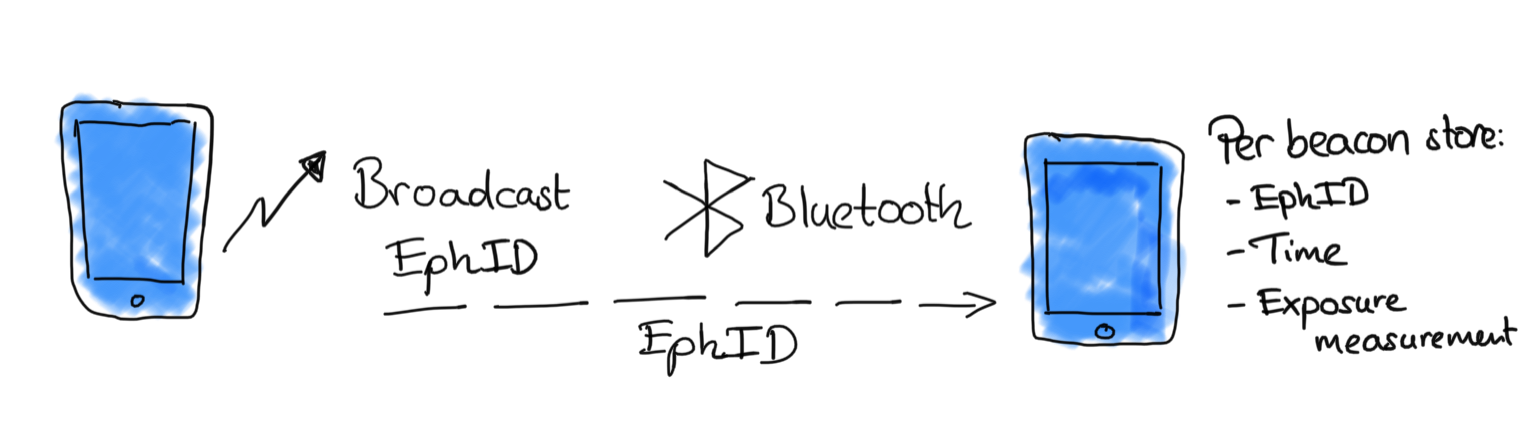
\includegraphics[width = 0.8\textwidth]{figs/storing_beacons.png}
\label{fig:storing_beacons}
\caption{Processing and storing of observed beacons.}
\end{figure}



\hypertarget{low-cost-decentralized-proximity-tracing}{%
\subsection{Low-cost decentralized proximity
tracing}\label{low-cost-decentralized-proximity-tracing}}

In this section, we present a low-cost protocol that has good privacy
properties and very small bandwidth requirements.

\hypertarget{setup}{%
\paragraph{Setup}\label{setup}}

\emph{Initial seed generation.} Let t be the current day. Smartphones
generate a random initial daily seed SK\textsubscript{t} for the current
day t. We assume days correspond to UTC days.

\hypertarget{creating-ephemeral-ids-ephids}{%
\paragraph{Creating ephemeral IDs
(EphIDs)}\label{creating-ephemeral-ids-ephids}}

\emph{EphID Generation}. Each day, smartphones rotate their secret day
seed SK\textsubscript{t} by computing

SK\textsubscript{t} = H( SK\textsubscript{t - 1} ),

where H is a cryptographic hash function. The smartphone will use the
seed SK\textsubscript{t} during day t to generate EphIDs.

To avoid location tracking via broadcast identifiers, devices should
frequently change the ephemeral identifier EphID that they broadcast to
other devices. We refer to the duration for which a device broadcasts
the same EphID as an \textbf{epoch}. The length of an epoch, in minutes,
is a configurable system parameter that we denote as L.

At the beginning of each day t, smartphones locally generate a list of n
= (24 * 60)/L new EphID\textsubscript{i}s to broadcast during day t.
Given the day seed SK\textsubscript{t}, each device computes

EphID\textsubscript{1} \textbar\textbar{} ... \textbar\textbar{}
EphID\textsubscript{n} = PRG( PRF(SK\textsubscript{t}, ``broadcast
key'') ),

where PRF is a pseudo-random function (e.g., HMAC-SHA256), ``broadcast
key'' is a fixed, public string, and PRG is a pseudorandom generator
(e.g. AES in counter mode) producing n * 16 bytes, which we split into
16-byte chunks to obtain the n ephemeral Bluetooth identifiers EphID for
the day.

Smartphones pick a random order in which to broadcast the EphIDs during
the day. Each EphID\textsubscript{i} is broadcast for L minutes.

\hypertarget{local-storage-of-observed-ephids-and-seeds-skt}{%
\paragraph{\texorpdfstring{Local storage of observed EphIDs and seeds
SK\textsubscript{t}
}{Local storage of observed EphIDs and seeds SKt }}\label{local-storage-of-observed-ephids-and-seeds-skt}}

For each received beacon, phones store:

\begin{itemize}
\item
  \begin{quote}
  The received ephemeral Bluetooth identifier EphID.
  \end{quote}
\item
  \begin{quote}
  The exposure measurement (e.g., signal attenuation).
  \end{quote}
\item
  \begin{quote}
  The day on which this beacon was received (e.g., ``April 2'').
  \end{quote}
\end{itemize}

Note that an EphID could be received multiple times and will result in
multiple entries in the database (Figure \ref{fig:storing_beacons}). For efficient storage, we
propose to group these entries by EphID, resulting in 36 bytes per
EphID. Given a very conservative estimate of 140k different observations
over the course of 14 days (i.e., if epochs are 15 minutes, these are
100 different people observed per epoch), this would require around 6.1
MB.

In addition, each device stores the seeds SK\textsubscript{t} it
generated during the past 14 days. This parameter (i.e., 14 days), which
defines the maximum period for which any data (both observed and
generated EphIDs)is stored on the device, is a system parameter and is
determined by guidance from health authorities.

\hypertarget{decentralized-proximity-tracing-1}{%
\paragraph{Decentralized proximity
tracing}\label{decentralized-proximity-tracing-1}}

Once the health authority has authorised the proximity tracing for a
confirmed COVID-19 positive user (Figure \ref{fig:pt_lowcost}, step 1), the user can
instruct their phone to send to the backend the seed SK\textsubscript{t}
and the day t corresponding to the first day in which the user was
considered to be contagious (Figure \ref{fig:pt_lowcost}, step 2). The start date of the
contagious window t can either be determined by the health authority or
the user might be trusted to manually enter this day.\footnote{``Secure
  Upload Authorisation for Digital Proximity Tracing'', The DP-3T
  Project,
  \href{https://github.com/DP-3T/documents/blob/master/DP3T\%20-\%20Upload\%20Authorisation\%20Analysis\%20and\%20Guidelines.pdf}{{https://github.com/DP-3T/documents/blob/master/DP3T\%20-\%20Upload\%20Authorisation\%20Analysis\%20and\%20Guidelines.pdf}}}
Epidemiologists estimate that for COVID-19 the contagious window starts
1 to 3 days before the onset of symptoms.

After reporting the seed SK\textsubscript{t} and day t for the first day
of the contagious window, the smartphone deletes SK\textsubscript{t}. It
then picks a completely new random seed and commences broadcasting
EphIDs derived from this new seed. This ensures that after uploading
their past seed, users do not become trackable. Recall that our system
does not attempt to track users after reporting a diagnosis because we
assume users act responsibly. The new seed will thus only be uploaded if
necessary, i.e., if after a second positive diagnosis the user is
considered contagious.

Given the seed SK\textsubscript{t}, everyone can compute all ephemeral
identifiers EphID broadcast by the COVID-19 positive user, starting from
day t by repeating the process described in
\protect\hyperlink{creating-ephemeral-ids-ephids}{{EphID generation}}
above.

The backend collects the pairs (SK\textsubscript{t},t) of COVID-19
positive users. Phones periodically download these pairs (Figure \ref{fig:pt_lowcost},
step 3). Each smartphone uses this pair to reconstruct the list of
EphIDs of a diagnosed person for each day t' and checks (1) if it has
observed any beacon with one of these EphIDs on day t' and (2) that such
observations occurred before the corresponding seed SK\textsubscript{t}
was published.\footnote{To facilitate this check, the smartphone
  temporarily stores a more precise receive timestamp of all the beacons
  it received after the last download from the server. Once all
  downloads from the server have been processed, the phone coarsens this
  timestamp for all past observations.} Restricting the matching to a
specific day limits replay attacks in which malicious users redistribute
captured EphIDs and ensures more efficient lookups.

For each matching recorded beacon (e.g., a beacon with an EphID that was
transmitted by a user who reported a positive diagnosis), the beacon's
receive time and exposure measurement are taken into account for the
exposure risk computation (Figure \ref{fig:pt_lowcost}, step 4) and
\protect\hyperlink{exposure-estimation}{{Section 4}}.

\begin{figure}\centering
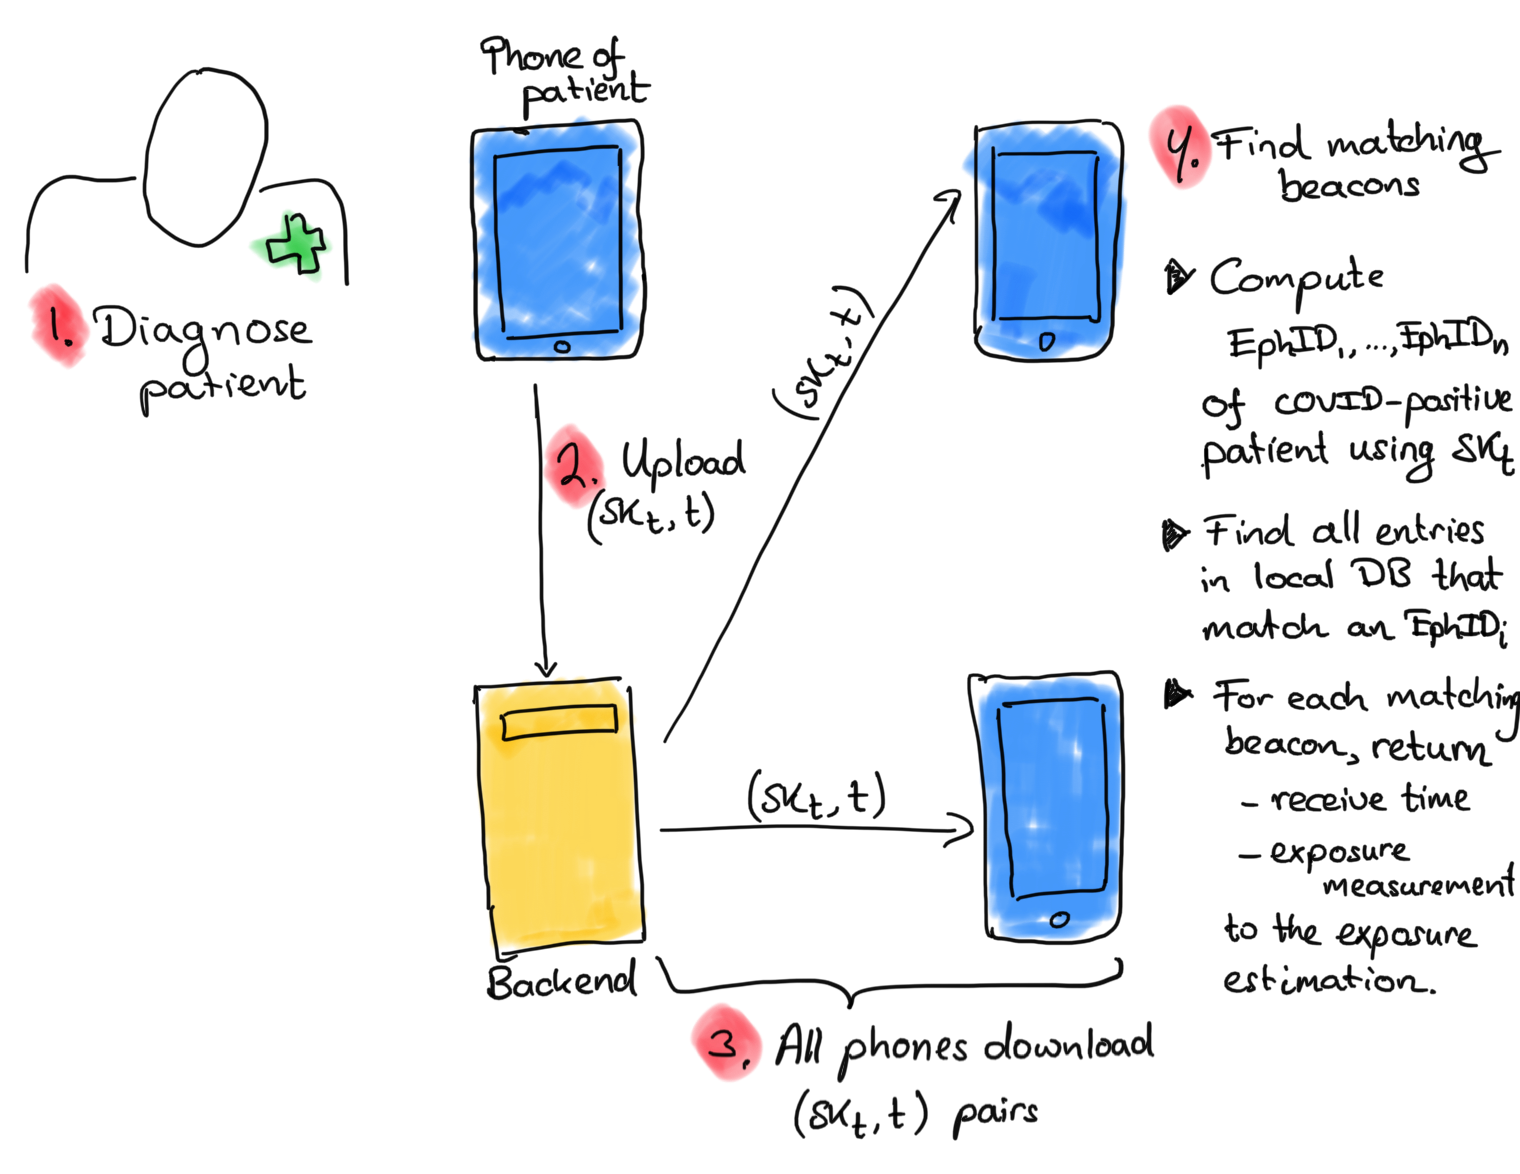
\includegraphics[width=5.27083in,height=3.83887in]{figs/PT-lowcost.png}
\caption{Proximity tracing process.}
\label{fig:pt_lowcost}
\end{figure}


\paragraph{Scalability}\label{scalability}

For each user who reports a positive diagnosis, the backend needs to
store a 32-byte seed and a 2-byte day counter for the duration of the
contagious window. Storage cost at the backend is therefore not a
problem. Throughout the day, smartphones download the 32-byte seeds and
2-byte day counters of newly diagnosed patients. This data is static and
can therefore be effectively served through a content delivery network
(CDN).


\subsection{Unlinkable decentralized proximity tracing}\label{unlinkable-decentralized-proximity-tracing}

In this section, we present a variant of the low-cost design in the
previous section that offers better privacy properties than the low-cost
design at the cost of increased bandwidth. This design does not
disseminate a list containing the seeds of users who have reported a
positive diagnosis. Instead, the ephemeral identifiers of COVID-19
positive users are hashed and stored in a Cuckoo filter, which is then
distributed to other users.

This design choice offers several advantages. It prevents adversaries
from linking the ephemeral identifiers of COVID-19 positive users (see
privacy analysis for details), and it enables COVID-19 positive users to
redact, after a positive diagnosis, identifiers corresponding to
sensitive locations, times, or periods in which users are certain they
have not been in contact with other people, e.g. while they were alone
or behind a window.

\hypertarget{setup-1}{%
\paragraph{Setup}\label{setup-1}}

No setup is needed.

\hypertarget{generating-ephemeral-ids}{%
\paragraph{Generating ephemeral IDs}\label{generating-ephemeral-ids}}

As in the low-cost design, smartphones broadcast each ephemeral
identifier EphID during one epoch of fixed duration L. Epochs i are
encoded relative to a fixed starting point shared by all entities in the
system.

Smartphones generate the ephemeral identifier EphID\textsubscript{i} for
each epoch i as follows. The smartphone draws a random 32-byte per-epoch
seed seed\textsubscript{i} and sets:

EphID\textsubscript{i} = LEFTMOST128( H( seed\textsubscript{i} ) ),

where H is a cryptographic hash function, and LEFTMOST128 takes the
leftmost 128 bits of the hash output. Smartphones store the seeds
corresponding to all past epochs in the last 14 days. They delete older
seeds. As before, the maximum storage period is a system parameter and
is determined with guidance from health authorities.

\hypertarget{local-storage-of-observed-ephids}{%
\paragraph{Local storage of observed
EphIDs}\label{local-storage-of-observed-ephids}}

For each observed beacon the smartphone stores:

\begin{itemize}
\item
  \begin{quote}
  The hashed string H(EphID \textbar\textbar{} i), where H is a
  cryptographic hash function, and EphID the identifier of the beacon,
  and i is the epoch in which the beacon is received. (Note that this
  differs from the low-cost design, in which the phone stores the raw
  EphID.)
  \end{quote}
\item
  \begin{quote}
  The exposure measurement (e.g., signal attenuation)
  \end{quote}
\item
  \begin{quote}
  The day in which this beacon was received (e.g., ``April 2'').
  \end{quote}
\end{itemize}

We include the epoch i in the hash to ensure that replaying an EphID
outside the epoch in which it was originally broadcast can never cause a
fake at-risk event (regardless of whether the EphID corresponds to a
person who later reports a positive diagnosis).

For efficiency of storage, we propose to group these entries by hashed
string. A single entry then requires around 52 bytes. Given a very
conservative estimate of 140k different observations over the course of
14 days (i.e., 100 people observed per epoch), this would require around
6.9 MB of local storage.

\hypertarget{decentralized-proximity-tracing-2}{%
\paragraph{Decentralized proximity
tracing}\label{decentralized-proximity-tracing-2}}

In case of a positive diagnosis, users can instruct their device to
upload a representation of the EphIDs produced by the smartphone during
the contagious window. Unlike in the low-cost design, the user first has
the option to \emph{redact} identifiers by choosing the set I of epochs
for which they want to reveal their identifiers. For example, the user
may want to exclude Monday morning and Friday night. The phone then
uploads the set \{(i, seed\textsubscript{i})\} for all epochs i in I.
Requiring seed\textsubscript{i} rather than the resulting EphID, ensures
that malicious users cannot claim somebody else's EphID as their own
(see
\protect\hyperlink{security-analysis-of-unlinkable-design}{{security
analysis}}).

Periodically (e.g., every 2 hours), the backend creates a new Cuckoo
filter F and for each pair (i, seed\textsubscript{i}) uploaded by a
COVID-19 positive user it inserts

H ( LEFTMOST128( H( seed\textsubscript{i} ) ) \textbar\textbar{} i)

into the Cuckoo filter F, i.e., the hashed string H(EphID
\textbar\textbar{} i) where EphID = LEFTMOST128( H(
seed\textsubscript{i} ) ) as above. The outer hash-function is needed
for security. The backend publishes the filter. All smartphones download
it.

Each smartphone uses the filter F to check if in the past (i.e., before
the corresponding filter F was published), it has observed any of the
EphIDs reported by COVID-19 positive users. The phone checks if any of
its stored hashes are included in the filter F.

For each matching beacon (e.g., a beacon with a recorded hashed
identifier that was transmitted by a user who reported a positive
diagnosis), the beacon's receive time and exposure measurement are
provided to the exposure risk computation
(\protect\hyperlink{exposure-estimation}{{Section 4}}).

Cuckoo filters have a low, but non-zero, probability of false positives,
that is reporting that they contain an element that was not in the input
set. In order to avoid unnecessarily alarming users, we select the
parameters of the Cuckoo filter such that false positives are highly
unlikely to occur even with heavy usage of the system over a number of
years. In the scalability calculation below, we configure the filter to
produce one false positive in a million users over a period of 5 years.

The use of a Cuckoo filter hides the set of ephemeral identifiers of
COVID-19 positive users from the general public. The system uses a
Cuckoo filter in conjunction with inputs that are obtained from
cryptographic hashes of random values (the seeds, concatenated with
timestamps). The inputs to the filter are sparse in a large set, i.e.,
the set of all possible inputs (128-bit strings). These two factors
makes enumeration attacks against the filter an unattractive attack
vector for adversaries, while still making it possible for users who
have observed particular ephemeral identifiers to check for their
inclusion in the filter. Attacks that attempt to reverse the filter and
directly recover inputs from values held in the filter do not result in
exposure of ephemeral IDs because of the extra layer of hashing
performed on ephemeral IDs before entering them into the filter.

\hypertarget{scalability-1}{%
\paragraph{Scalability}\label{scalability-1}}

This design requires more bandwidth and storage than in the low-cost
design. The backend needs to store Cuckoo filters containing the hashed
identifiers of COVID-19 positive users during the contagious period.
Smartphones regularly download new cuckoo filters containing the latest
hashed identifiers of COVID-positive patients. This data is static and
can therefore be effectively served through a content delivery network.
The computational cost on the phone is likely smaller than in the
low-cost design, as phones only need to do one lookup per stored hashed
identifier per cuckoo filter sent by the backend.

\hypertarget{hybrid-decentralized-proximity-tracing}{%
\subsection{Hybrid decentralized proximity
tracing}\label{hybrid-decentralized-proximity-tracing}}

In this section, we present a hybrid design that combines ideas from the
low-cost design and the unlinkable design. In this design, phones
generate random seeds for each time window (for example, of length 2
hours) and use these seeds similar to the low-cost design to generate
ephemeral identifiers for all epochs within that time window. Users
upload seeds only if they are relevant to exposure estimation by other
users.

Depending on the length of the time window, this design offers much
better protection against linking ephemeral identifiers of COVID-19
positive users than the low-cost design and enables a user to redact
time windows. The protection against tracking is weaker than the
unlinkable design, but this scheme has a smaller bandwidth requirement.

This design is very similar to the Google/Apple design.\footnote{See
  \href{https://www.apple.com/covid19/contacttracing/}{{https://www.apple.com/covid19/contacttracing/}}}
The Google/Apple design uses one seed to generate the ephemeral
identifiers of that day, and thus corresponds to the special case where
windows are 1 day long. In that configuration, the advantages with
respect to the low-cost design are smaller. We recommend a time window
of 2 or 4 hours depending on the bandwidth availability in the region.

\hypertarget{setup-2}{%
\paragraph{Setup}\label{setup-2}}

No setup is needed.

\hypertarget{generating-ephemeral-ids-1}{%
\paragraph{Generating ephemeral IDs}\label{generating-ephemeral-ids-1}}

As in the previous designs, smartphones broadcast EphID during an epoch
of fixed duration L. We group consecutive epochs into a time window w.
The length of a time window can range from 10 minutes to a full day and
needs to be an integer multiple of L.

At the start of each time window w, smartphones pick a new random
16-byte seed seed\textsubscript{w}. Given the seed seed\textsubscript{w}
for window w, each device computes

EphID\textsubscript{w,1} \textbar\textbar{} ... \textbar\textbar{}
EphID\textsubscript{w,n} = PRG( PRF(seed\textsubscript{w},
``DP3T-HYBRID'') ),

where PRF is a pseudo-random function (e.g., HMAC-SHA256),
``DP3T-HYBRID'' is a fixed and public string, and PRG is a pseudorandom
generator (e.g. AES in counter mode) producing n * 16 bytes, which we
split into 16-byte chunks to obtain the n ephemeral Bluetooth
identifiers EphID for the window w.

Smartphones pick a random order in which to broadcast the n ephemeral
Bluetooth identifiers within the window w. Each EphID\textsubscript{i}
is broadcast for L minutes.

\hypertarget{local-storage-of-observed-ephids-1}{%
\paragraph{Local storage of observed
EphIDs}\label{local-storage-of-observed-ephids-1}}

Smartphones locally record the observed beacons, similar to the low-cost
design. For each received beacon the phone stores:

\begin{itemize}
\item
  \begin{quote}
  The received ephemeral Bluetooth identifier EphID,
  \end{quote}
\item
  \begin{quote}
  The exposure measurement,
  \end{quote}
\item
  \begin{quote}
  The time window w in which the EphID was received.
  \end{quote}
\end{itemize}

For efficiency of storage, we propose to group these entries by EphID,
resulting in 36 bytes per EphID. Given a very conservative estimate of
observing 140k different EphIDs over the course of 14 days (i.e., if
epochs are 15 minutes, this would be 100 people observed per epoch),
this would require 4.8 MB of local storage.

\hypertarget{decentralized-proximity-tracing-3}{%
\paragraph{Decentralized proximity
tracing}\label{decentralized-proximity-tracing-3}}

In case of a positive diagnosis, users can instruct their device to
upload the relevant seeds seed\textsubscript{w} generated by the
smartphone during the contagious period. If the phone did not observe
any EphID sufficiently close to be considered as an exposure during a
time window w, it does not upload the corresponding seed
seed\textsubscript{w} for efficiency. As in the unlinkable design, the
user additionally has the option to \textbf{redact} identifiers, by
choosing the set W of windows for which they want to reveal their
identifiers. For example, the user may want to exclude windows for
Monday morning and Friday night. The phone then uploads the set \{(w,
seed\textsubscript{w})\} for all windows w in W.

The backend collects pairs (w, seed\textsubscript{w}) of COVID-19
positive users. Phones periodically download these pairs. Each
smartphone uses these pairs to reconstruct the list of EphIDs of
COVID-19 positive users for each window w' and checks if it has observed
any of these EphIDs during window w' \emph{in the past} (i.e., before
the corresponding seed seed\textsubscript{w} was published). Restricting
the matching to a specific time window limits replay attacks in which
malicious users redistribute captured EphIDs and ensures more efficient
lookups.

For each matching recorded beacon (e.g., a beacon with an EphID that was
transmitted by a COVID-19 positive user), the beacon's receive time and
exposure measurement are given as inputs to the exposure risk
computation, see \protect\hyperlink{exposure-estimation}{{Section 4}}.


\paragraph{Scalability}
This design requires more bandwidth and storage than the low-cost
design, but less than the unlinkable design. The backend needs to store
the (w, seed\textsubscript{w}) pairs corresponding to COVID-19 positive
users. Smartphones regularly download all new pairs. This data is static
and can therefore be effectively served through a content delivery
network.

The download cost depends on the length of the window and how many
windows can be automatically omitted by the smartphone when uploading
seeds. See Figure \ref{fig:scale_hybrid} for a comparison. See the next section for how we
computed these numbers.


\begin{figure}\centering
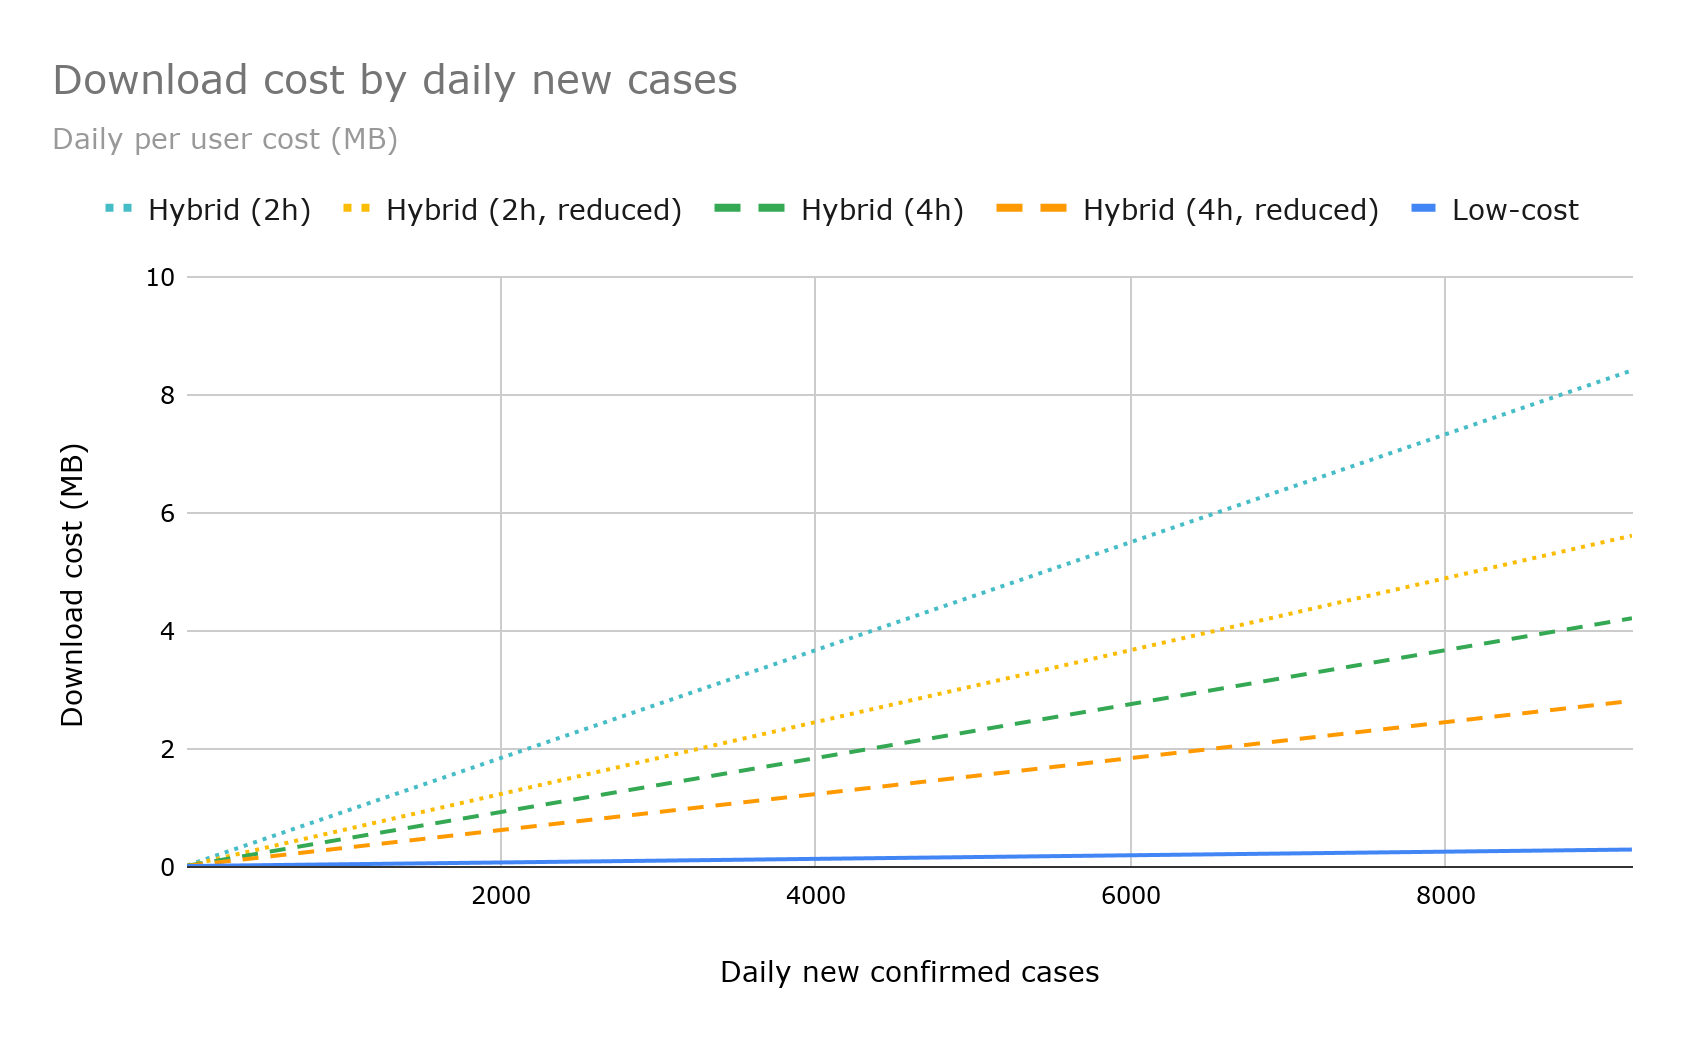
\includegraphics[width=0.8\textwidth]{figs/scalability_hybrid.png}
\label{fig:scale_hybrid}
\caption{\textbf{Scalability of the hybrid design}. Comparison of the
daily download cost per user (MB) depending on the number of new
confirmed cases per day for different upload configurations of the
hybrid design. We compare the download cost for different lengths of the
time window w under two different assumptions. In the ``normal'' case,
COVID-positive users upload seeds for all windows. In the ``reduced''
case their smartphone automatically omits the seeds for windows with a
total length of 8 hours (e.g., because they were alone during that time
and the phone did not detect any contacts).}
\end{figure}


\subsection{Scalability}\label{scalability-3}

All three designs benefit from the use of a content delivery network
(CDN). Smartphones of COVID-positive patients upload a small amount of
data to the backend server. The backend server regularly redistributes
this data to all other smartphones using a CDN. The daily download size
scales linearly with the number of COVID-positive patients in all three
designs. We assume a contagious window of 5 days and 15-minute epochs.

\begin{itemize}
\item
  \begin{quote}
  In the low-cost design, the server needs to distribute one
  (SK\textsubscript{t}, t) pair per diagnosed patient. This requires 36
  bytes per patient.
  \end{quote}
\item
  \begin{quote}
  In the unlinkable design, the server needs to distribute 5 * 96 hashed
  strings per diagnosed patient. When using a well-tuned Cuckoo filter,
  this requires 2880 bytes per patient.
  \end{quote}
\item
  \begin{quote}
  In the hybrid design, we assume windows of 2 to 4 hours. The server
  must therefore distribute 5 * 6 or 5 * 12 seeds per diagnosed patient.
  This requires 480 to 960 bytes per user. Users that can redact 8 hours
  of windows only need to send 5 * 4 and 5 * 8 seeds, requiring 320 and
  640 bytes respectively.
  \end{quote}
\end{itemize}

See Figure \ref{fig:comp_decentralized} for the resulting daily download cost for smartphones.
Table DC shows specific values based on peak rates in several countries.

We expect that proximity tracing systems, even when deployed in large EU
countries, will operate in the range of up to 2000 new cases a day. At
the time of writing, all large EU countries see less than 1500 new cases
a day. We expect that if the rate of new cases increases, countries will
take policy measures to restrict the infection rates. Thus, we expect
the download cost to never exceed the single-digit requirement.

\begin{figure}\centering
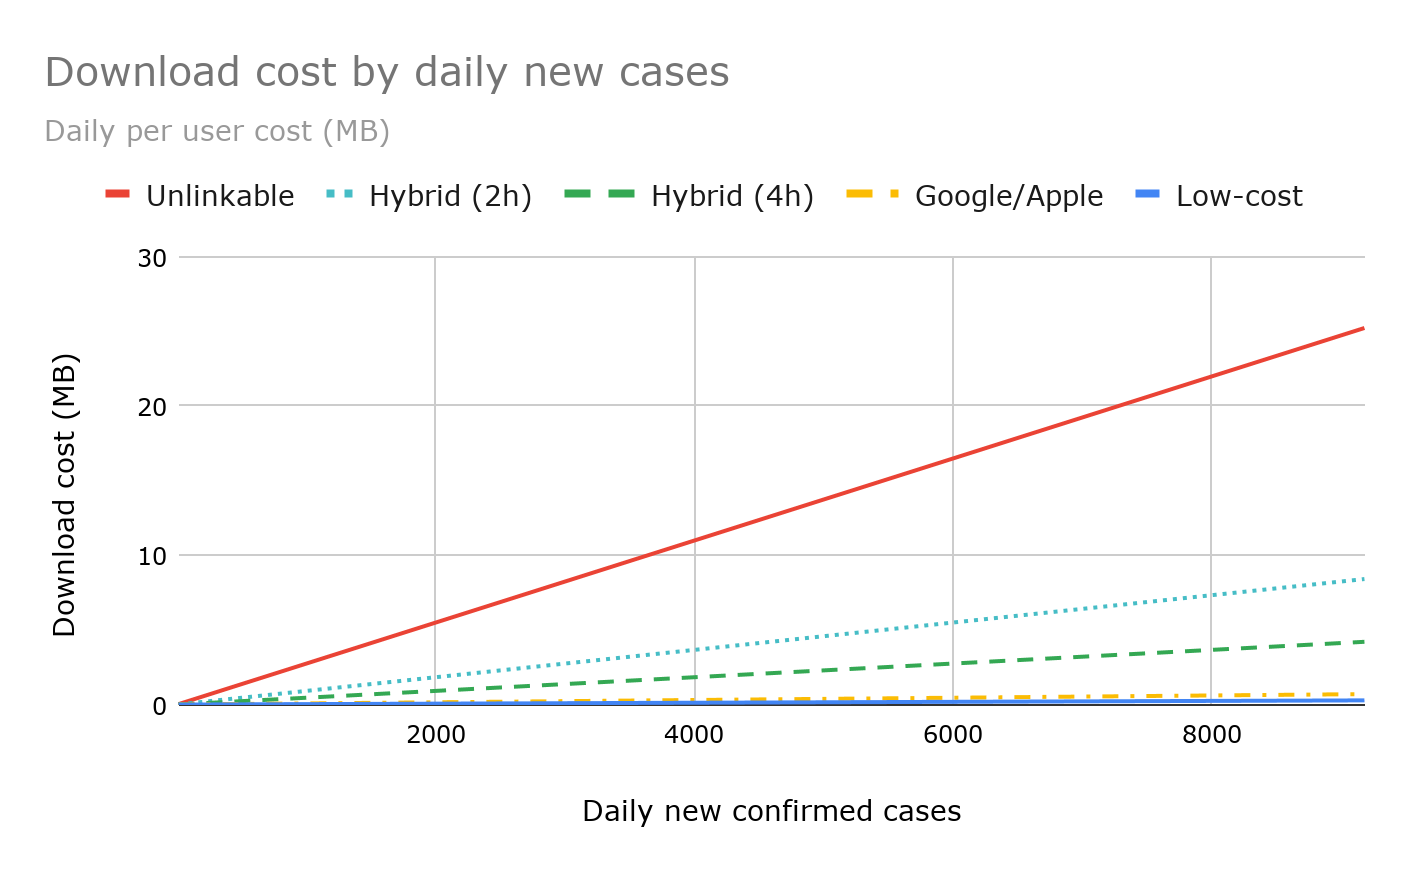
\includegraphics[width=0.8\textwidth]{figs/comparison_decentralized.png}
\label{fig:comp_decentralized}
\caption{Comparison of the daily download cost per user (MB)
by number of new confirmed cases per day for different decentralised
proximity tracing designs.}
\end{figure}


\begin{tabular}[]{@{}llll@{}}
\toprule
& \textbf{Low-cost (MB)} & \textbf{Unlinkable (MB)} & \textbf{Hybrid
(4h) (MB)}\tabularnewline
\midrule
\textbf{Switzerland (8M)} & & &\tabularnewline
1390 cases & 0.04 & 3.82 & 0.64\tabularnewline
58 cases & 0.00 & 0.16 & 0.03\tabularnewline
\textbf{Germany (83M)} & & &\tabularnewline
6294 cases & 0.19 & 17.29 & 2.88\tabularnewline
933 cases & 0.03 & 2.56 & 0.43\tabularnewline
\textbf{France (67M)} & & &\tabularnewline
7578 cases & 0.23 & 20.81 & 3.47\tabularnewline
708 cases & 0.02 & 1.94 & 0.32\tabularnewline
\textbf{Spain (42M)} & & &\tabularnewline
9181 cases & 0.28 & 25.22 & 4.20\tabularnewline
849 cases & 0.03 & 2.33 & 0.39\tabularnewline
\textbf{Italy (60M)} & & &\tabularnewline
6557 cases & 0.20 & 18.01 & 3.00\tabularnewline
1402 cases & 0.04 & 3.85 & 0.64\tabularnewline
\bottomrule
\end{tabular}

\section{Interoperability in decentralised proximity tracing
systems}\label{interoperability-in-decentralised-proximity-tracing-systems}

Effective proximity tracing systems must be interoperable across
borders. Phones of users visiting foreign countries, whether it is for
work, or for leisure, must be able to capture beacons from users in
countries that they visit and include beacons of COVID-19 diagnosed
patients in those countries in their exposure computation. Likewise,
residents of a country must be able to receive notifications if a
visitor to their country is diagnosed with COVID-19.

All three proposed designs support interoperability between different
operators of different regions. Interoperability is possible as long as
these operators use one of the decentralized designs proposed in this
document. To interoperate with a specific protocol, the smartphone
application must be able to process tracing data published for that
protocol. That is, the application must run as many protocols as it
needs to interoperate with.

To enable cross-border interoperability, backend servers of different
regions (e.g., countries, or states) must exchange data. We propose the
following mechanisms, explained in detail in other documents.\footnote{For
  an overview see ``Interoperability of decentralized proximity tracing
  systems across regions'' retrieved from
  \href{https://drive.google.com/file/d/1mGfE7rMKNmc51TG4ceE9PHEggN8rHOXk}{{https://drive.google.com/file/d/1mGfE7rMKNmc51TG4ceE9PHEggN8rHOXk}}
  on 20 May 2020. A more detailed specification is provided here:
  ``Decentralized Proximity Tracing: Interoperability Specification''.
  The DP-3T Team (18 May 2020). Retrieved on 20 May 2020 from:
  \href{https://github.com/DP-3T/documents/blob/master/DP3T\%20-\%20Interoperability\%20Decentralized\%20Proximity\%20Tracing\%20Specification\%20(Preview).pdf}{{https://github.com/DP-3T/documents/blob/master/DP3T\%20-\%20Interoperability\%20Decentralized\%20Proximity\%20Tracing\%20Specification\%20(Preview).pdf}}}

First, when visiting a region, users enter the region into their phone.
If a user visits a region frequently, e.g., workers commuting across
borders, both regions can be permanently added to their phones. Phones
use the list of visited regions to retrieve any proximity tracing data
published by that region's backend for up to 14 days after the end of
the users' visit. The way in which proximity data are published differs
by protocol. For the low-cost design, this is a list of
(SK\textsubscript{t},t) pairs, for the unlinkable design this is the
cuckoo filter, and for the hybrid design this is the list of (w,
seed\textsubscript{w})pairs. The phones then follow the
protocol-specific procedures to match observed EphIDs, which they then
feed into the exposure risk computation described in the next section.

Second, to ensure all contacts of diagnosed users are notified, when a
user is diagnosed with COVID-19, the phone will ask the user for
recently visited regions. When uploading the seeds to the server, the
phones also supply the list of visited regions. The backend
authenticates the upload and then redistributes the uploaded tracing
data to all visited regions. As a result, users in those regions will
download this data and can determine if they observed any of the
visitors' EphIDs.


\section{Exposure estimation}\label{exposure-estimation}

The goal of the exposure estimation is to estimate the duration of the
smartphone owner's exposure to COVID-19 positive users in the past. This
measurement serves as a proxy for the level of exposure to the
SARS-CoV-2 virus. Local health authorities determine the exposure
threshold for when a user should receive a notification. A prolonged
exposure to the virus does not imply that the virus has been
transmitted. However, the notification serves as a trigger for
precautionary interventions recommended by local health authorities,
such as testing or quarantine.

To compute exposure, the smartphone proceeds as follows. First, if
necessary, it downloads the latest parameters provided by the health
authority. Next, it takes all matches reported by the proximity tracing
system for the past 14 days and estimates the exposure. In Switzerland,
for instance, for each day, the phone combines the exposure measurements
(e.g. signal attenuations) of all matches corresponding to that day, to
compute a per-day exposure score.\footnote{Details on the exposure
  estimation from BLE proximity measurements will be provided soon as
  separate documentation}

If the exposure score is above the threshold determined by the health
authority, the smartphone displays a notification that the user has been
exposed to the virus through prolonged physical proximity to COVID-19
positive individuals. The notification advises the user on what to do
and where to find more information. The details of the messages
displayed, including the rate of repeated notifications and their
content, need to be designed in close collaboration with health
authorities and mental health experts.


\section{Security and privacy considerations}\label{security-and-privacy-considerations}

In this section, we analyse the privacy and security properties of the
three decentralised proximity tracing protocols introduced in this
document. We have published a separate, far more extensive, risk
evaluation of digital proximity tracing systems\footnote{``Privacy and
  Security Risk Evaluation of Digital Proximity Tracing Systems'', The
  DP-3T Project,
  \href{https://github.com/DP-3T/documents/blob/master/Security\%20analysis/Privacy\%20and\%20Security\%20Attacks\%20on\%20Digital\%20Proximity\%20Tracing\%20Systems.pdf}{{https://github.com/DP-3T/documents/blob/master/Security\%20analysis/Privacy\%20and\%20Security\%20Attacks\%20on\%20Digital\%20Proximity\%20Tracing\%20Systems.pdf}}}
that includes the class of decentralised systems our three designs
belong to.

\subsection{Threat model}\label{threat-model}

In this section, we describe the adversaries that we take into account
when carrying out the security and privacy analysis. For each of these
adversaries, we describe their capabilities and the kind of risk they
pose for the system. In the next section, we analyze the security and
privacy of the system with respect to these adversaries.

\textbf{Regular user.} A typical user of the system that is assumed to
be able to install and use the application by navigating its user
interface (UI). They exclusively look at information available via the
app's UI to infer private information about other users.

\textbf{Tech-savvy user} (Blackhat/Whitehat hacker, NGOs, Academic
researchers, etc.)\textbf{.} This user has access to the system via the
mobile App. In addition, she can set up (BT, WiFi, and Mobile) antennas
to eavesdrop locally. Finally, she can decompile/modify the app, and she
has access to the backend source code.

\begin{itemize}
\item
  (Whitehat hacker) Will investigate the App code, the information in
  the phone, and will look at what information is exchanged with the
  server (using an antenna or software installed on the phone, e.g.,
  \href{https://haystack.mobi/}{{Lumen}}) or broadcast via Bluetooth
  (passive).
\item
  (Malicious) Can DOS the system (targeted or system-wide), deviate from
  protocols, and actively broadcast Bluetooth identifiers.
\end{itemize}

\textbf{Eavesdropper} (Internet Service Provider, Local System
administrators, Bluetooth sniffer)\textbf{.} They can observe network
communication (i.e., source and destination of packages, payload, time)
and/or BLE broadcast messages.

\begin{itemize}
\item
  \begin{quote}
  (Network adversary) Can use observed network traffic to attempt to
  determine the state of a user (e.g., whether they are at-risk,
  COVID-19 positive, etc.).
  \end{quote}
\item
  \begin{quote}
  (Local Bluetooth BLE Sniffer) Can observe local Bluetooth broadcasts
  (possibly with a powerful antenna to cover a wider area) and try to
  trace people.
  \end{quote}
\end{itemize}

It should be noted however that in many instances, for individuals or
companies to use data in this way, or to collect data about passers-by
to try and estimate their infection status based on the announced
identifiers, will fall foul of a range of existing national and European
laws around data protection, ePrivacy and computer misuse.

\textbf{Health authority.} Receives information about COVID-19 positive
users as part of their normal operations to diagnose patients. The
health authority learns information about at-risk people only when these
at-risk people themselves reach out to the health authority (e.g., after
receiving a notification from their app).

\textbf{Backend and App developers.} Can access all data stored at the
servers. Moreover, the backend can query data from the mobile app in the
same way that it would do during normal operations (in our designs, it
can only change the data downloaded by the smartphones). They could also
change the code of their backend software and the code of the mobile
apps (including parameters related to proximity tracing). We assume they
will not modify the mobile app because such action would be detectable.
They can combine and correlate information, request information from
apps, combine with other public information to learn (co-)location
information of individuals.

\textbf{State-level adversary} (Law enforcement, intelligence agencies,
etc)\textbf{.} Has the combined capabilities of the tech-savvy user and
the eavesdropper. In addition, a state-level adversary can obtain
subpoenas that give them the capabilities of the health authority, or
the backend. Their goal is to obtain information about the population or
to target particular individuals. They may be interested in past
information, already stored in the system, or future information that
will enable them to trace target individuals based on observed EphIDs.

\textbf{Unlimited-budget adversary.} An adversary with an unlimited
budget, e.g., large organizations and (foreign) nation states, has the
capabilities of tech-savvy users but can deploy these at a much larger
scale. Additionally, such an adversary might be able to gain control
over the project's infrastructure such as the backend. The goals of this
adversary might be to learn information about the population or
individuals (cf. a state-level adversary) or to disrupt the proximity
tracing system, resulting in a form of denial of service. One form of
disruption is to try cause a sizable part of the population to receive
fake at-risk notifications by deploying antennas in public locations
(e.g., airports, train stations, shopping malls, or parliament
buildings) and relaying messages far and wide. This relay attack
increases the chances of ``at risk'' contacts for the targeted
population because their phones will perceive proximity where there is
none.


\subsection{Privacy}\label{privacy}

\subsubsection{Privacy concerns}\label{privacy-concerns}

\textbf{Social graph.} The social graph describes social relationships
between users. Each node in the graph represents an individual user and
an edge connecting two nodes indicates that there is a social
relationship between the two users. A proximity tracing system does not
need to provide information on the social graph to any party to fulfill
its primary purpose.

\textbf{Interaction graph.} The interaction graph reflects close-range
physical interactions between users. A labelled edge indicates an
interaction between two adjacent users at a specific time. Knowledge of
this graph is not necessary for proximity tracing nor for analyzing the
spread of SARS-CoV-2. Therefore, \emph{no party} needs to learn the
interaction graph.

\textbf{Location traceability.} To perform proximity tracing, location
traces (e.g. GPS coordinates) are not required. Therefore, no party in
the system needs to have access to them or be able to easily trace
individuals based on the BLE signals that the app broadcasts.

\textbf{At-risk individuals.} At-risk individuals are people who have
recently been in contact with somebody who has tested positive for
COVID-19. At-risk individuals need to know that they have been exposed
to the virus so that they can take appropriate measures. No other party
in the system needs to learn this information, other than when the
notified user contacts and identifies herself to the health authority.

\textbf{COVID-19 positive status.} Only the user and the health
authority need to know that the user has tested positive for COVID-19.
No other party in the system needs to learn this information. In
particular, app users do not need to know which of the individuals with
whom they have been in contact have tested positive.

\textbf{(Highly) Exposed locations.} The system does not need to reveal
any information about the locations that COVID-19 positive individuals
have visited or the number of positive cases that have visited a
specific location (e.g., to build a heat map of exposures). Proximity
tracing can be performed without any party learning this information.


\subsubsection{Privacy analysis of low-cost
design}\label{privacy-analysis-of-low-cost-design}

\textbf{Social graph.} The low-cost design does not reveal any
information to any entity. Any two users involved in a contact may learn
this contact's existence from the system, but this was already known to
them.

\textbf{Interaction graph.} The system does not reveal any information
about the interaction between two users to any entity. The EphIDs
revealed by COVID-19 positive users do not allow any inference about the
people they have been in contact with to anyone except those contacts.
The system thus prevents outside parties from learning the interaction
graph.

\textbf{Location traceability.} In our low-cost design, the EphIDs of
all users are unlinkable, and only the smartphone that generated them
knows the corresponding seeds SK\textsubscript{t}. When the phone's
owner is diagnosed with SARS-Cov-2 and gives permission, the phone
publishes to the backend the seed SK\textsubscript{t} corresponding to
the first contagious day. After disclosing this information, the phone
will generate a new seed at random. Given the seed SK\textsubscript{t}
of the first contagious day, the EphIDs of a COVID-19 positive user are
linkable from the start of the contagious window until the time of
upload (at which point the phone picks a new seed).

As a result, tech-savvy users, eavesdroppers, and state-level
adversaries can \emph{locally} track infected patients during the (past)
window in which the identifiers broadcasted via Bluetooth are linkable.
To do so, the attacker uses strategically placed Bluetooth receivers and
recording devices to receive EphIDs. The app's Bluetooth broadcasts of
non-diagnosed users and COVID-19 positive users outside the contagious
window remain unlinkable.

\textbf{At-risk individuals.} The seeds revealed to the server by
COVID-19 positive users \emph{are independent of} their contacts, i.e.,
the people they interacted with. They therefore do not give any
information about people at risk to any party other than the at-risk
individuals themselves.

\textbf{COVID-19 positive status.} Any proximity tracing system that
informs a user that she has been in contact with a confirmed positive
case inherently reveals a piece of information to the person at risk:
one of the people they interacted with has tested positive for COVID-19.

A curious or malicious adversary might attempt to exploit this and other
information in the system to identify the COVID-positive individuals
with whom they have been in close proximity.

A curious user who only uses the standard interface of the app, cannot
learn which of their contacts has tested positive because the app in
normal operation does not reveal any information other than that the
user was exposed at some point in the past. Such a curious user can only
learn which of their contacts has tested positive if they learn this
fact on an out-of-band channel (e.g., the COVID-positive person informs
them, they observe the person going to the hospital, a common friend
reveals the COVID-positve status, etc.).

A proactive tech-savvy adversary can abuse any proximity tracing system
to identify individuals who have reported a positive diagnosis to the
system and that she has been in close proximity with. This risk is a
consequence of the basic proximity tracing functionality. The attack can
be executed regardless of implementation and proximity tracing protocol
(BLE or otherwise). It only relies on the single bit of information that
any proximity tracing system must reveal --- whether you have been
exposed to a confirmed COVID-19 positive case.

To reveal an individual's COVID-19 positive status, the adversary must
(1) keep a detailed log of who they saw and when, (2) register many
accounts in the proximity tracing system, and (3) use each account for
proximity tracing during a short time window. When one of these accounts
is notified, the attacker can link the account identifier back to the
time-window in which the contact occurred to learn when she was in close
proximity to an individual who reported a positive diagnosis\textbf{.}
The attacker can correlate this information with their detailed
interaction log to narrow down who in their list of contacts is COVID-19
positive. In some cases, the adversary might even be able to single out
an individual. This attack \textbf{is inherent to any proximity-based
notification system,} as the adversary only uses the fact that they are
notified together with additional information gathered by their phone or
through other means.\footnote{For further details on this attack see
  ``Privacy and Security Risk Evaluation of Digital Proximity Tracing
  Systems'', The DP-3T Project,
  \href{https://github.com/DP-3T/documents/blob/master/Security\%20analysis/Privacy\%20and\%20Security\%20Attacks\%20on\%20Digital\%20Proximity\%20Tracing\%20Systems.pdf}{{https://github.com/DP-3T/documents/blob/master/Security\%20analysis/Privacy\%20and\%20Security\%20Attacks\%20on\%20Digital\%20Proximity\%20Tracing\%20Systems.pdf}}}

In decentralized proximity tracing systems, such as the three designs we
propose in this white-paper, tech-savvy adversaries can learn when they
were in close proximity to a COVID-19 positive individual without having
to create multiple accounts. To determine when they interacted with a
COVID-19 positive individual, they \textbf{proactively modify the
app}\footnote{We note that in some schemes such modifications would
  preclude the App from accessing measurement data entirely when using
  the Google and Apple API.} to store detailed logs of which EphID they
received and when, and cross reference this list with the EphIDs
reported by COVID-19 positive cases downloaded from the backend server.
They then correlate exposure times with their log of who they saw to
reveal which individuals they have been in contact with reported a
positive diagnosis.

The low-cost design allows an adversary to \textbf{link} the EphIDs
reported by COVID-19 positive cases, i.e. to learn which Bluetooth
identifiers belong to the same device\emph{\textbf{.}} COVID-19 positive
individuals upload a single seed SK\textsubscript{t} that enables others
to reconstruct, and thus link, a person's EphIDs for the entire
contagious period. Due to the linkability of reported EphIDs, an
attacker can \textbf{combine observations} at different times to
identify who reported a positive diagnosis to the system\emph{.} For
example, the attacker might learn that the infected person she saw at
10:11AM is \emph{the same} as the one she saw at 14:14PM. While she may
have encountered many different people at each time, the intersection
might be much smaller. This further increases the likelihood that the
attacker can successfully single out a COVID-19 positive individual.

Tech-savvy users can also conduct a retroactive attack in which they
attempt reidentification based on linkage and stored data, without the
need to collect additional information in advance. The retroactive
attacker only uses information stored by the app and auxiliary knowledge
about the whereabouts of individuals during the contagious period. The
data stored in the app provides coarse timing information when a
specific EphID has been observed, e.g., per day in the low-cost design.
A tech-savvy adversary could leverage this information to single out a
COVID-19 positive individual based on matching observed EphIDs to
background knowledge of whom the adversary was with during this time
window. A combination of multiple time windows might be enough to
uniquely identify to whom the reported EphIDs belong. However, since
smartphones broadcast the daily set of EphIDs in random order, the
attacker cannot use the published seeds SK\textsubscript{t} to narrow
down this coarse time-window. This decreases the likelihood that she
will be able to successfully identify the COVID-19 positive individual
in her contact list.

To \textbf{re-identify} an individual who has reported a positive
diagnosis for COVID-19 to the system, an adversary needs to be able to
\textbf{associate an identity} to the auxiliary information they have
collected. For instance, a tech-savvy adversary who collects a detailed
log of who they saw when needs to associate identities to each log
entry. Without knowing the identities, the adversary cannot learn who
tested positive. We can divide individuals the adversary interacts with
into three groups depending on whether she will be able to reveal their
identities or not:

\begin{itemize}
\item
  \begin{quote}
  \emph{Close individuals}: Family, friends, or colleagues with whom the
  adversary spends long periods of time. If these people received a
  positive diagnosis, they \emph{will inform the adversary personally
  about their diagnosis} if they have spent time together. It is common
  practice that the authorities ask COVID-19 patients to notify any
  contact person at risk they remember.
  \end{quote}
\item
  \begin{quote}
  \emph{Routine-sharing individuals}: People who share an activity with
  the adversary, such as riding a bus every day, supermarket tellers,
  etc. COVID-19 positive individuals in this group will likely not
  remember having been in contact with them and therefore will not (and
  cannot) notify the adversary.
  \end{quote}
\item
  \begin{quote}
  \emph{Anonymous individuals:} People that the adversary sees
  sporadically and whose identities are unknown to the adversary.
  \end{quote}
\end{itemize}

As close individuals will reveal themselves, there is no extra
information that an adversary can gain about the COVID-19 positive
status of this group by exploiting the app. Anonymous COVID-19 positive
users cannot be easily identified. Their privacy is only at risk if the
adversary deploys additional (costly) means to associate identities with
collected background knowledge. For instance, the adversary could
attempt to combine data from surveillance cameras with facial
recognition techniques to learn who is whom. The main group that is thus
at risk through identification attacks is routine-sharing individuals.

We stress that in any case, having been close to an COVID-19 positive
person is not proof of causality regarding transmission of the virus.
Moreover, it is worth noting that reidentifying individuals and
inferring their health status as a private entity without their
permission would likely violate data protection law and, potentially,
computer misuse law, which would further increase the cost and risk of
undertaking this attack.

The pattern associated with the upload of identifiers to the server
would reveal the COVID-19 positive status of users to network
eavesdroppers (ISP or curious WiFi provider) and tech-savvy adversaries.
If these adversaries can bind the observed IP address to a more stable
identifier such as an ISP subscription number, then they can
de-anonymize the confirmed positive cases. This can be mitigated by
using dummy uploads. These dummy uploads provide plausible deniability
to actual users' uploads, i.e., given an upload an observer cannot
distinguish if it corresponds to an actual positive or a dummy. To avoid
revealing which uploads were dummies to an adversary that polls the
backend to learn if the list of ephemeral identifiers was updated, the
backend should batch updates and only publish them in designated
download slots.\footnote{Details on the generation of dummy traffic will
  be provided in future documentation.}

The backend server learns the IP address of COVID-19 positive users when
they upload (a representation of) their EphIDs. If this adversary can
bind the observed IP address to a more stable identifier, they can
de-anonymize the confirmed positive patients. To reduce the risk, we
recommend that the backend not log IPs.

\emph{Mitigations}\textbf{.} In the current setting, retroactive
attackers can link beacons received at different, coarse times to aid in
identifying COVID-19 positive users. The amount of information available
to such an attacker can be reduced by running the proximity tracing
protocol either inside a privileged OS-level module\footnote{This is the
  approach taken by the Google/Apple API.} or inside a local trusted
execution environment (TEE). These approaches isolate the proximity
tracing protocol and the data they collect from users and malicious
apps. The protocols running in the isolated environment would only
output for each matching beacon: the corresponding exposure measurement
(e.g., the attenuation) and a coarse time. The app then computes the
exposure score (see \protect\hyperlink{exposure-estimation}{{Section
4}}). As a result, retroactive attackers can only learn the number of
beacons of infected patients received each day but can no longer link
beacons by the same COVID-19 positive patient.

By itself, this approach does not protect against tech-savvy users that
proactively modify their device to collect beacons and then compute
matching COVID-19 positive beacons using the public list of COVID-19
positive EphIDs. However, when using TEEs to isolate the proximity
protocol, the system can be extended to hide this public list from
tech-savvy users, ensuring that they \textbf{cannot} \textbf{recognize}
COVID-19 positive beacons. To protect against tech-savvy users when
using TEEs, the backend encrypts the list of seeds so that this list can
only be decrypted \emph{inside} the TEE. Each TEE downloads and decrypts
the list of infected EphIDs and finds the matching beacons by cross
referencing the list of infected EphIDs with the collected beacons. The
TEE then returns to the app, for each day, a vector of the exposure
measurements that enable the app to determine the user's exposure. As
long as the TEE remains secure, tech-savvy users do not learn the EphIDs
of COVID-19 positive patients.

Modern phones are equipped with TEEs that are used to harden smartphone
kernels against attacks and to store cryptographic seeds. TEEs require
buy-in from mobile platform providers (Apple, Google) and, for Android,
the device manufacturers (Samsung, Huawei, etc.). The TEEs are well
protected and difficult to attack even for tech-savvy users. While it is
not impossible to leak this information, it is unlikely. We think such a
mitigation is worthwhile in a later version of the proximity tracing
system to further increase privacy guarantees. Other mitigation
techniques could include the use of Private Information Retrieval and
Private Set Intersection techniques, although current implementations
may bring severe performance penalties.

Such technical measures as well as non-technical measures (e.g., banning
modified applications from the market) could be introduced in case that
the identification of COVID-19 positive individuals would become a
threat to the system operation and to the users. The introduction of
such measures depends on the overall risk assessment.

Finally, we note that if a small, cautious or misinformed portion of the
population is concerned with these attacks and decides not to
participate, this will not greatly impair the effectiveness of the
deployment. As long as a large fraction of the population runs the app,
the number of at-risk identifications will be large enough to
significantly reduce the rate of transmission.

\textbf{(Highly) Exposed locations.} A powerful tech-savvy adversary
operating its own BLE equipment from a single location can collect
EphIDs within 20-100m range, depending on the phone output power and
environment. When combining this list with the EphIDs that can be
computed from the SKs downloaded to the phone, an adversary could learn
whether any COVID-19 positive user has visited the location in a small
radius of 50m. Furthermore, the adversary could reveal how many distinct
diagnosed persons have visited the location in the past.

\hypertarget{privacy-analysis-of-unlinkable-design}{%
\subsubsection{Privacy analysis of unlinkable
design}\label{privacy-analysis-of-unlinkable-design}}

The unlinkable design provides overall better privacy properties at the
cost of increased bandwidth. The two designs provide the same level of
protection for the social and interaction graph. We address the
remaining differences point by point.

\textbf{Location traceability.} In the unlinkable design, the EphIDs
remain unlinkable for all users against a local attacker. This
unlinkability also holds for COVID-19 positive patients so long as the
server is honest. However, if the server is malicious, then it can infer
which ephemeral identifiers belong to a COVID-19 positive user through
timing information or other metadata created when ephemeral identifiers
are uploaded to the server. The use of anonymous communications could
mitigate this threat.

\textbf{At-risk individuals.} As in the low-cost design, the seeds
revealed to the server by users who have received a positive diagnosis
\emph{are independent of} their contacts. Hence, they do not give any
information about people at risk.

The rest of the analysis is the same as for the low-cost design.

\textbf{COVID-19 positive status.} The unlinkable design reduces the
linkability of the EphIDs reported by a COVID-19 positive user. Compared
to the low-cost design, this reduces the likelihood that a proactive or
retroactive tech-savvy adversary can identify which of their contacts
has reported a positive diagnosis through linkage attacks. The adversary
can no longer combine observations at multiple points of time to single
out a COVID-19 positive individual.

Retroactive attackers can extract little information from the records
stored on the phone. For each beacon, the phone only stores the hashed
string, a coarse receive time (e.g., the day on which the beacon was
received) and the exposure measurement. Retroactive attackers cannot
recover a more detailed receive time, and thus only learn the total
count of COVID-19 positive beacons for each day.

However, a proactive tech-savvy adversary can still modify their
application to learn when she has been in close proximity to a confirmed
positive case. As described in our detailed privacy risk
evaluation,\footnote{See ``Privacy and Security Risk Evaluation of
  Digital Proximity Tracing Systems'', The DP-3T Project,
  \href{https://github.com/DP-3T/documents/blob/master/Security\%20analysis/Privacy\%20and\%20Security\%20Attacks\%20on\%20Digital\%20Proximity\%20Tracing\%20Systems.pdf}{{https://github.com/DP-3T/documents/blob/master/Security\%20analysis/Privacy\%20and\%20Security\%20Attacks\%20on\%20Digital\%20Proximity\%20Tracing\%20Systems.pdf}}}
this attack can be executed in any proximity tracing system by using
multiple accounts. It cannot be avoided.

The unlinkable design enables COVID-19 positive individuals to redact
periods of time that they consider sensitive and for which they prefer
not to disclose their contacts. This can alleviate concerns in a
close-knit or small community in which users may be concerned that
community members learn of their positive diagnosis through the app,
instead of being informed in person.

\textbf{(Highly) Exposed locations.} As in any practical BLE-based PT
system, an adversary could identify locations that have been visited by
COVID-positive users in the past. However, as EphIDs cannot be linked to
a single device, it is more difficult for the adversary to learn how
many distinct cases visited the location.


\subsubsection{Privacy analysis of hybrid
design}\label{privacy-analysis-of-hybrid-design}

The hybrid design provides privacy properties similar to the low-cost
and the unlinkable design. There are two major differences between the
hybrid and the low-cost design.

\begin{enumerate}
\def\labelenumi{\arabic{enumi})}
\item
  \begin{quote}
  The hybrid design controls the linkability of the ephemeral
  identifiers reported by COVID-19 positive users and restricts
  linkability to short to medium-length time windows.
  \end{quote}
\item
  \begin{quote}
  The hybrid design allows users who report a positive diagnosis to
  redact identifiers for specific time windows before sharing them with
  other devices.
  \end{quote}
\end{enumerate}

These two differences affect the privacy properties of the hybrid design
in the following ways:

\textbf{COVID-19 positive status.} Proactive and retroactive linkage
attacks by tech-savvy adversaries aim to reveal the COVID-19 positive
status of individuals they have been in close proximity with. To learn
this information, the adversary needs to extract from the system
\emph{at which times} they have been in contact with a COVID-19 positive
user. They can then correlate this information to auxiliary knowledge
about who they saw when to identify individuals who reported a positive
diagnosis. If the adversary can link ephemeral identifiers, i.e.,
associate multiple of the EphIDs reported by COVID-19 positive users to
the same individual, the adversary can combine observations from
different time frames to single out individuals. The hybrid design
restricts the linkability of reported EphIDs to a time window w. This
reduces the likelihood that the adversary can successfully narrow down
the group of contacts who might have tested positive.

In comparison to the unlinkable design, the medium-term linkability of
EphIDs implies the hybrid design provides slightly less protection
against proactive and retroactive identification attacks. We note
though, that as in all decentralized designs discussed in this white
paper, the proactive tech-savvy user must modify their application to
record receive times.

The hybrid design allows COVID-19 positive users to decide not to share
their broadcast identifiers for certain time windows. This further
reduces the likelihood of successful identification attacks as the
adversary cannot use auxiliary information for the redacted time frames
to reveal the identity of diagnosed users.

Retroactive attackers can extract some information from the records
stored on the phone. For each beacon, the phone stores the EphID, a time
and the exposure measurement. Because EphIDs from the same COVID-19
positive patient are linkable during a time window, the retroactive
attacker can estimate contact duration with a single COVID-19 positive
patient for each time window.\footnote{This retroactive attack does not
  work when using the Google/Apple API as it does not expose received
  EphID to any application or user.}

\textbf{(Highly) Exposed locations.} An adversary is less likely to be
able to learn the number of positive cases who visited a specific
location because of the restricted linkability of ephemeral identifiers.
The adversary can link EphIDs for the duration of a time window but
cannot link identifiers of the same individual across multiple time
windows.

\subsection{Security}\label{security}

\subsubsection{Security concerns}\label{security-concerns}

\textbf{Fake exposure events.} A fake exposure event could make a person
believe that they are at risk, even though they have never been exposed
to a diagnosed user. Attackers could try to generate fake exposure
events to trigger false alerts, e.g. by relaying or broadcasting EphIDs
at large scale. This would violate the authenticity requirement of the
system.

\textbf{Suppressing at-risk contacts:} There is a risk that either a
COVID-19 positive user or the backend server could prevent other
individuals from learning they are at risk, e.g., by modifying the app's
local storage. This violates the integrity of the system and would lead
to an increased health risk for at-risk individuals who rely on the
system for alerts.

\textbf{Prevent contact discovery:} A malicious actor could disrupt the
system, e.g. by jamming Bluetooth signals, and prevent contact
discovery.

\hypertarget{security-analysis-of-low-cost-design}{%
\subsubsection{Security analysis of low-cost
design}\label{security-analysis-of-low-cost-design}}

\textbf{Fake exposure events.} In all practical proximity tracing
systems based on Bluetooth-based exposure measurements, an adversary
with a powerful antenna can trigger false alerts of an exposure to a
COVID-19 positive person that do not reflect real-world proximity to a
positive-case person.

To cause false alarms, a malicious adversary simply places her proximity
tracing device in a crowded area and hooks up a powerful transmitter to
\emph{artificially increase the range} of her Bluetooth contacts. As a
result, other devices located beyond 2 meters can interact with the
attacker's device and will perceive the attacker's device as
``near-by''. To complete the attack, the attacker must ensure that these
interactions between her device and other devices are flagged as
exposure events. To do so, the attacker either:

\begin{enumerate}
\def\labelenumi{\arabic{enumi}.}
\item
  \begin{quote}
  \textbf{Herself tests positive} and brings her device to the hospital
  when she gets tested (requiring the adversary to be infected).
  \end{quote}
\item
  \begin{quote}
  \textbf{Bribes a diagnosed person} to bring the attacker's device to
  the hospital instead of their own (or simply obtains the upload
  authorization code from them).
  \end{quote}
\item
  \begin{quote}
  \textbf{Hijacks/bribes the health authority} that authorises COVID-19
  positive individuals to trigger proximity tracing.
  \end{quote}
\item
  \begin{quote}
  \textbf{Compromises the backend server} that sends information or
  directly notifies users of the system.
  \end{quote}
\end{enumerate}

In the low-cost design, an attacker can record an individual's ephemeral
identifier and broadcast it to victims at a different location and/or
time, as long as it is \textbf{relayed on the same day}. If that
individual later receives a positive diagnosis, the victims will
incorrectly believe they have been exposed.

In the low-cost design, the seeds of COVID-19 positive users shared for
exposure calculation are bound to the day on which they were valid. This
prevents relay attacks in which the adversary attempts to relay an
individual's ephemeral identifiers with a delay of more than 24 hours.

An attacker could be motivated to claim another user's EphID as their
own and report that it should be included in the exposure risk
calculation. The low-cost design addresses this risk by requiring users
to upload the seeds SK\textsubscript{t} from which their EphIDs are
derived. As these EphIDs are derived from the seed using a cryptographic
hash function and a pseudo-random function, it is computationally
infeasible for an attack to learn another user's seed from observing
their broadcasts.

\textbf{Suppressing at-risk contacts.} Hiding at-risk contacts is
possible in any proximity tracing system. Infected users can choose to
not participate at all; to temporarily not broadcast Bluetooth
identifiers, or not to upload their data once diagnosed.

\textbf{Prevent contact discovery.} Any proximity tracing system based
on Bluetooth low energy is susceptible to jamming attacks by active
adversaries. Such jamming attacks will cause the normal recording of
EphIDs to stop working, hence preventing contact discovery. This is an
inherent problem of this approach.

\hypertarget{security-analysis-of-unlinkable-design}{%
\subsubsection{Security analysis of unlinkable
design}\label{security-analysis-of-unlinkable-design}}

The unlinkable design has the same security properties as the low-cost
design with respect to \textbf{suppressing at-risk contacts} and
\textbf{preventing contact discovery}.

\textbf{Fake exposure events.} As in all practical proximity tracing
systems based on BLE handshakes between personal smartphones, a powerful
adversary can cause false alarms through BLE range extension
attacks.\footnote{For further details on this general attack see
  ``Privacy and Security Risk Evaluation of Digital Proximity Tracing
  Systems'', The DP-3T Project,
  \href{https://github.com/DP-3T/documents/blob/master/Security\%20analysis/Privacy\%20and\%20Security\%20Attacks\%20on\%20Digital\%20Proximity\%20Tracing\%20Systems.pdf}{{https://github.com/DP-3T/documents/blob/master/Security\%20analysis/Privacy\%20and\%20Security\%20Attacks\%20on\%20Digital\%20Proximity\%20Tracing\%20Systems.pdf}}}

In the unlinkable design, ephemeral identifiers are cryptographically
linked to the \emph{epoch} in which they are broadcast. To create fake
exposure events, the attacker must therefore receive and rebroadcast
EphIDs \emph{within the same epoch.} Such an \textbf{``online'' relay
attack} is unavoidable in proximity tracing systems based on passive
Bluetooth advertisements.

As in the low-cost design, the EphID generation protocol of the
unlinkable design prevents an attacker from claiming another user's
EphID as their own. To do so, an attacker would have to be able to infer
a user's seed seedt from their broadcast identifier which is
computationally infeasible.

\subsubsection{Security analysis of hybrid
design}\label{security-analysis-of-hybrid-design}

The hybrid design has the same security properties as the low-cost
design with respect to the risks of suppressing at-risk contact and
preventing contact discovery.

\textbf{Fake exposure events.} As in all practical proximity tracing
systems based on BLE handshakes between personal smartphones, a powerful
adversary can cause false alarms through BLE range extension attacks.

In the hybrid design, EphIDs are linked to the valid time window of the
seed they were derived from. To create fake exposure events, the
adversary must therefore receive and broadcast EphIDs within the same
time window. This prevents relay attacks in which the adversary attempts
to relay an individual's ephemeral identifiers with a delay of more than
the length of a time window.

As in the low-cost design, the EphID generation protocol of the hybrid
design prevents an attacker from claiming another user's EphID as their
own. To do so, an attacker would have to be able to infer a user's seed
value seed\textsubscript{w} from their broadcast identifier which is
computationally infeasible.

\section{Protection from short-term and remote
eavesdropping at the physical layer}\label{protection-from-short-term-and-remote-eavesdropping-at-the-physical-layer}

In this section, we introduce an enhancement to the decentralised
proximity tracing solutions proposed in this document. It would also
apply to similar initiatives such as PACT and TCN,\footnote{For PACT,
  see Justin Chan et al. (2020)
  \href{https://arxiv.org/pdf/2004.03544.pdf}{{PACT: Privacy Sensitive
  Protocols and Mechanisms for Mobile Contact Tracing},} retrieved from:
  \href{https://covidsafe.cs.washington.edu/}{{https://covidsafe.cs.washington.edu/}}on
  20 May 2020. For TCN, see TCN Coalition (2020)
  \href{https://github.com/TCNCoalition/TCN}{{TCN Protocol},} retrieved
  from
  \href{https://github.com/TCNCoalition/TCN}{{https://github.com/TCNCoalition/TCN}}
  on 20 May 2020.} and the
\href{https://www.apple.com/covid19/contacttracing/}{{joint}} Apple and
Google Exposure Notification protocol.\footnote{See
  \href{https://www.apple.com/covid19/contacttracing/}{{https://www.apple.com/covid19/contacttracing/}}}

A shortcoming in most decentralized proximity tracing systems based on
the exchange of BT advertisements between devices is that a malicious
party who is willing to modify their app or deploy their own software is
able to record a proximity event \emph{\textbf{despite only being in
contact for a short amount of time or at a long distance}.} This
violates the requirement that the system provide \emph{\textbf{precise}}
data, i.e. only report exposure events that represent actual physical
proximity.

In particular, an attacker could attempt to gather a significant number
of EphIDs by deploying specialist equipment, either in high-traffic
locations or in a vehicle that can cover a wide area (``wardriving'').
The attacker can also deploy high gain, directional antennas to cover
wide areas, further increasing the range and selectivity of the attack.
The attacker can later see which of the recorded EphIDs correspond to
users who reported a positive diagnosis and use additional metadata such
as location, timing, video surveillance, etc. to infer their identities.

We note that for these enhancements to be efficient, changes in
low-level smartphone components (e.g., Bluetooth chips) are likely
necessary. We expect that without these changes, these enhancements will
have a non-negligible impact on battery life.


\subsection{EphID spreading with secret sharing}\label{ephid-spreading-with-secret-sharing}

To address these problems, we introduce an enhancement to our system:
EphID \emph{Spreading With Secret Sharing}.

In a nutshell, this enhancement spreads each ephemeral identifier EphID
across low-power beacons using a \emph{\textbf{k-out-of-n secret sharing
scheme}}. Instead of transmitting each EphID within a single beacon, we
encode it into n shares, such that each receiver needs to receive at
least k shares to reconstruct the EphID. There are a number of secret
sharing techniques that could be used for this purpose. We are currently
running experiments to determine which is the most robust scheme for the
scenarios in which these systems are to be deployed.

\begin{figure}\centering
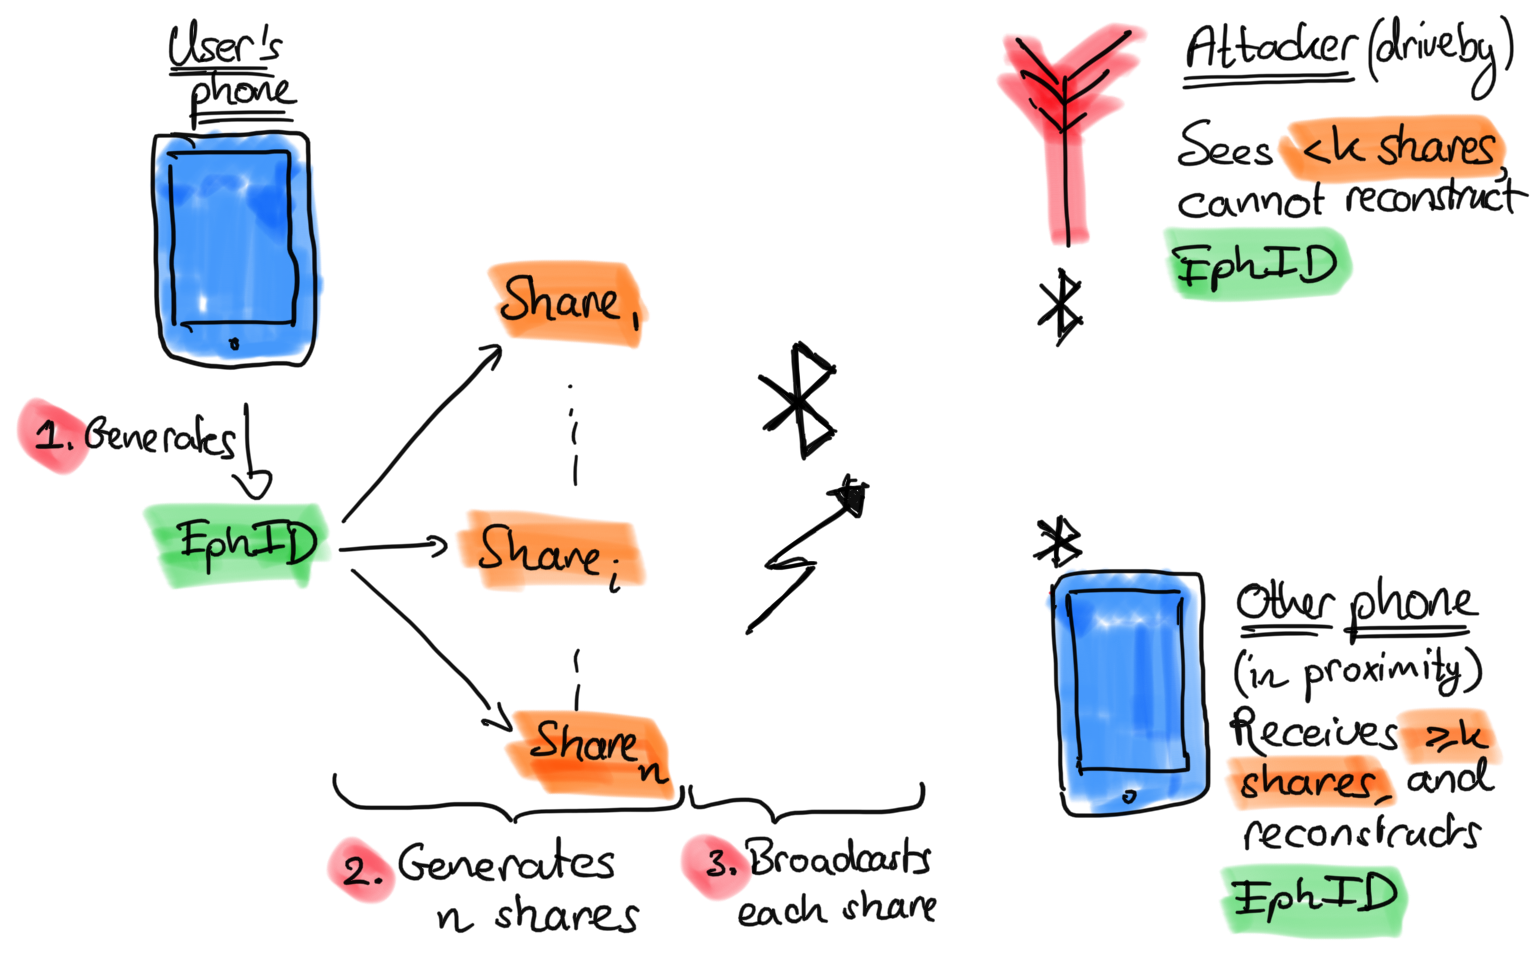
\includegraphics[width=0.8\textwidth]{figs/ephid_spreading.png}
\caption{EphID spreading with secret sharing.}
\end{figure}

In our earlier designs, each device divides time into epochs and picks a
random EphID\textsubscript{i} for each epoch i. The EphID is transmitted
several times during the epoch and each broadcast contains the whole
EphID. The broadcast frequency depends on manufacturer- and
implementation-specific details.

With this enhancement, each broadcast contains shares of the EphID. If
EphID is to be retransmitted within an epoch, new shares are generated.
In the simplest case, however, the number n of shares can be set to
equal the number of broadcasts that the device makes within an epoch. We
stress that this enhancement, even with the spread of the EphIDs, should
not have a significant impact on battery life. It requires no additional
transmission or reception over the basic designs, and the additional
computation is minimal.


\subsection{Tuning the trade-off between privacy and
utility}\label{tuning-the-trade-off-between-privacy-and-utility}

\emph{Tuning privacy parameters.} Setting the value k requires careful
consideration. A system must receive enough beacons during the contact
interval (as determined by epidemiologists) to receive k shares and
register a contact. A smaller k thus increases the robustness of the
system in normal operation. However, the larger the value of k, the
longer an adversary is forced to shadow a victim in order to collect a
sufficient number of beacons to reconstruct the EphID. Hence, the
proposed number k of shares is a trade-off between privacy and the
ability to record short contacts.

\emph{Eavesdropping from a distance.} Spreading EphID across beacons not
only protects against eavesdropping by adversaries who are only briefly
collocated with their victim, but it also makes eavesdropping from a
distance much harder. The requirement to successfully receive multiple
broadcasts increases the asymmetry between a legitimate receiver in
proximity and a malicious eavesdropper at a distance. An eavesdropper
who is placed further away will typically experience a worse channel to
the transmitter and a higher packet loss.

If we assume an attacker without access to specialised equipment and
with reasonable assumptions on the broadcast transmission power,
frequency, and probability of successful reception, we can select k, n
such that a close by, legitimate user within 5 meters would have a very
high probability of successfully receiving an EphID within a reasonable
contact time threshold of five minutes (\textgreater99.9\%), but an
attacker attempting to eavesdrop from 16 meters away would have a small
probability of success (\textless1\%). An attacker using specialised
hardware would be able to improve their odds either by increasing their
probability of successful reception or by cryptographic analysis of the
malformed broadcasts.

To achieve the appropriate balance between the desired range of
reception of EphIDs (epidemiologically relevant) and the resilience to
eavesdropping, we need to select the right combination of transmission
power, transmission frequency, and required number k of reconstruction
shares. We expect these parameters to be configurable and determined by
further experiments, functional requirements, and risk assessment. The
use of ultra-low or low power beacons will likely best protect the
privacy of the users and facilitate proximity detection.

Our scheme can be integrated within a ranging technique or used in
addition to existing (e.g., RSSI-based) ranging. In the latter case,
ranging would use a different epoch identifier that is different but
linked to the EphID that the device is broadcasting. If supported by BLE
chipsets, this scheme could be further enhanced by in addition
distributing the shares across three BLE advertisement channels.

\hypertarget{comparison-with-centralized-approaches}{%
\section{Comparison with centralized
approaches}\label{comparison-with-centralized-approaches}}

We classify two key functionalities in proximity tracing systems that
are decentralized in our schemes:

\begin{itemize}
\item
  \begin{quote}
  Ephemeral identifier generation: Ephemeral identifiers broadcast via
  Bluetooth are generated on the phone.
  \end{quote}
\item
  \begin{quote}
  Exposure estimation: The estimation of the exposure is computed
  locally on the phone.
  \end{quote}
\end{itemize}

We now compare the security and privacy properties of the decentralized
approaches presented above with schemes in which both operations are
centralized, and with schemes in which seeds are generated on phones but
COVID-exposure estimation is centralized.

\subsection{Centralized identifier generation and exposure
estimation}\label{centralized-identifier-generation-and-exposure-estimation}

In approaches in which both identifier generation and COVID-exposure
estimation are centralized, such as ROBERT,\footnote{Inria PRIVATICS and
  Fraunhofer AISEC (19 April 2020)
  \href{https://github.com/ROBERT-proximity-tracing/documents/blob/master/ROBERT-specification-EN-v1_0.pdf}{\emph{{ROBERT:
  ROBust and privacy presERving proximity Tracing}}}. Retrieved from
  \href{https://github.com/ROBERT-proximity-tracing/}{{https://github.com/ROBERT-proximity-tracing/}}
  on 19 May 2020.} PEPP-PT-NTK,\footnote{PEPP-PT (20 April 2020)
  \href{https://github.com/pepp-pt/pepp-pt-documentation/blob/master/10-data-protection/PEPP-PT-data-protection-information-security-architecture-Germany.pdf}{\emph{{Data
  Protection and Information Security Architecture: Illustrated on
  German Implementation}}}. Retrieved from
  \href{https://github.com/pepp-pt/}{{https://github.com/pepp-pt/}} on
  19 May 2020.} and OpenTrace/BlueTrace/TraceTogether,\footnote{Jason
  Bay, Joel Kek, Alvin Tan, Chai Sheng Hau, Lai Yongquan, Janice Tan,
  Tang Anh Quy (9 April 2020)
  \href{https://bluetrace.io/static/bluetrace_whitepaper-938063656596c104632def383eb33b3c.pdf}{\emph{{BlueTrace:
  A privacy-preserving protocol for community-driven contact tracing
  across borders}}}. Retrieved from
  \href{https://bluetrace.io/}{{https://bluetrace.io/}} on 19 May 2020.}
a central server estimates a user's likelihood of COVID-exposure,
instead of the user's smartphone in decentralized designs. Depending on
the system, the server notifies the at-risk users (PEPP-PT-NTK,
OpenTrace) or users query the server about their status (ROBERT).

In all these systems, the central server holds a long-term
pseudo-identifier for every user and uses it to derive ephemeral
pseudo-identities (EphIDs) that are pushed to the smartphones.

The smartphones broadcast the EphIDs received from the central server
and record the EphIDs transmitted by near-by smartphones. Smartphones
\emph{locally store all} observed EphIDs together with their
corresponding proximity and duration. See Figure ZZ.

In case of a positive diagnosis, users can give permission for their
smartphone to send the recorded list of observations to the server to
enable proximity tracing.

\begin{figure}\centering
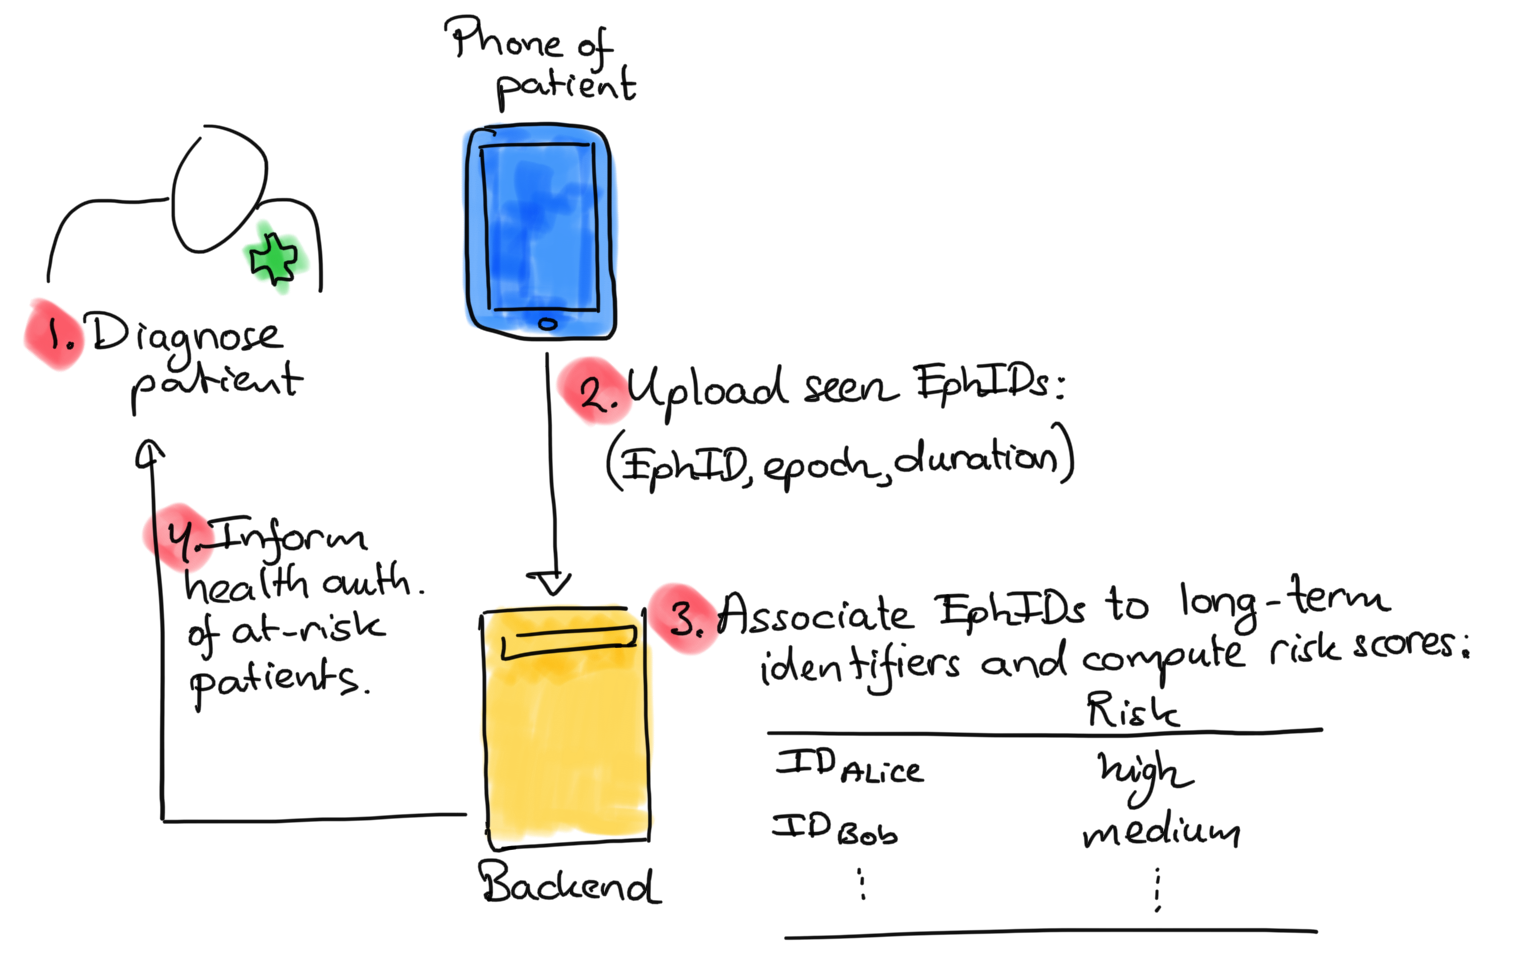
\includegraphics[width=0.8\textwidth]{figs/PT-central.png}
\caption{Processing and storing of observed EphIDs.}
\end{figure}


\subsubsection{Central proximity
tracing}\label{central-proximity-tracing}

\paragraph{PEPP-PT-NTK and OpenTrace}\label{pepp-pt-ntk-and-opentrace}

The PEPP-PT-NTK and OpenTrace backends execute the proximity tracing
process after a diagnosed user has uploaded their list of observations
{[}(EphID, epoch, duration){]} for the contagious window. The backend
recovers the long-term pseudo-identifiers of the at-risk users from the
reported observed EphIDs and triggers a process to notify them if their
exposure is high enough. See Figure ZY.

\begin{figure}\centering
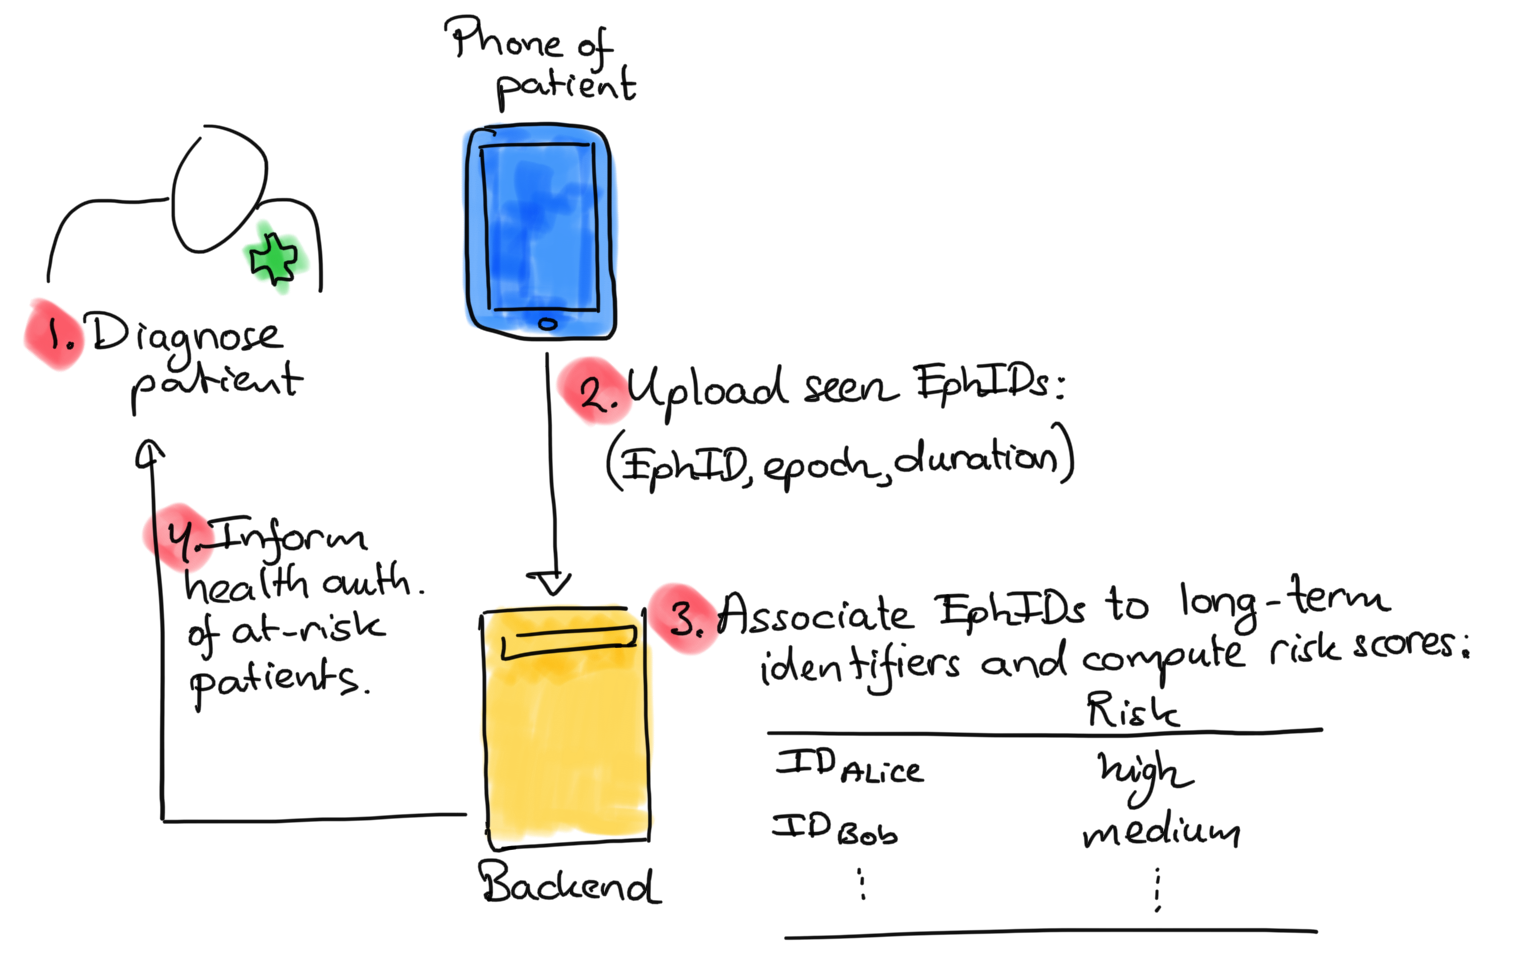
\includegraphics[width=0.8\textwidth]{figs/PT-central.png}
\caption{Proximity tracing for centralized PEPP-PT-NTK and OpenTrace designs. In ROBERT, the users instead query the backend.}
\end{figure}


\paragraph{ROBERT}\label{robert}

In the ROBERT system, the backend tracks the exposure of each user of
the system. As in PEPP-PT-NTK and OpenTrace, COVID-19 diagnosed patients
upload their observed EphIDs to the backend server. The backend server
associates these observed EphIDs to long-term pseudo-identifiers of
at-risk users. The backend uses the associated data to update the
exposure for each of the at-risk users.

Unlike PEPP-PT-NTK and OpenTrace, the backend does not notify patients.
Instead, smartphones of ROBERT users regularly query the backend to
request their exposure status. The backend answers whether the exposure
passed the threshold or not.

\hypertarget{local-identifier-generation-and-centralized-exposure-estimation}{%
\subsection{Local identifier generation and centralized exposure
estimation}\label{local-identifier-generation-and-centralized-exposure-estimation}}

Other approaches, such as DESIRE\footnote{Castellucia et al. (9 May
  2020) DESIRE: A third way for a European Exposure Notification System
  \href{https://github.com/3rd-ways-for-EU-exposure-notification/project-DESIRE/blob/master/DESIRE-specification-EN-v1_0.pdf}{{https://github.com/3rd-ways-for-EU-exposure-notification/project-DESIRE/blob/master/DESIRE-specification-EN-v1\_0.pdf}}
  on 19 May 2020.} instead generate identifiers on the phone, while
still estimating COVID-exposure centrally. Instead of broadcasting
self-contained, ephemeral identifiers, smartphones in DESIRE broadcast
ephemeral public keys that, when combined with others' public keys,
yield ephemeral identifiers EphIDs.

In case of a positive diagnosis, users can give permission for their
smartphone to send a version of the observed EphIDs to the backend to
enable proximity tracing.

\hypertarget{central-proximity-tracing-1}{%
\paragraph{Central proximity
tracing}\label{central-proximity-tracing-1}}

Smartphones regularly query the backend to request their current
exposure status. To enable the backend to compute this status, phones
upload a version of the EphIDs computed from all the encounters they had
in the relevant period. The server takes all observations reported of
these encounters {[}(EphID, epoch, duration){]} and estimates exposure.
If the exposure is long enough, the user receives a positive exposure
response. Otherwise, the user receives a negative.


\subsection{Privacy comparison}\label{privacy-comparison}

\textbf{Social graph.} In a system in which both identifiers and
COVID-exposure are computed centrally, the backend server can always
associate ephemeral broadcast identifiers with permanent
pseudo-identifiers for individual devices. If EphIDs are associated with
a long-term identifier (e.g., in PEPP-PT-NTK), the backend server can
reconstruct the social graph of users from the information shared by
COVID-19 positive users. The server can join subgraphs from different
positive cases to gain a comprehensive picture of the true underlying
social graph. Given other partial social graphs with identities, the
server can match its graph to the other graphs and reidentify nodes.

ROBERT and DESIRE propose to prevent the leakage of the social graph by
using an anonymous communication network to upload observed identifiers
in an unlinkable manner. In this way, the backend cannot associate
uploads to a user nor determine which identifiers were observed by the
same COVID-19 positive user. As a result, the backend cannot reconstruct
an infected user's contacts.

In separate documents, we show that (1) these mechanisms when applied to
ROBERT are ineffective and still allow reconstruction of the social
graph;\footnote{See, ``Security and privacy analysis of the document
  `ROBERT: ROBust and privacy-presERving proximity Tracing'\,'', The
  DP-3T Project, version 22 April 2020,
  {https://github.com/DP-3T/documents/blob/master/Security\%20analysis/ROBERT\%20-\%20Security\%20and\%20privacy\%20analysis.pdf}}
and (2) are difficult to realise in practice for DESIRE.\footnote{See,
  ``DESIRE: A Practical Assessment'', The DP3T Consortium, version 13
  May 2020,
  {https://github.com/DP-3T/documents/blob/master/Security\%20analysis/DESIRE\%20-\%20A\%20Practical\%20Assessment.pdf}}

\textbf{Interaction graph.} In a system in which both identifiers and
COVID-exposure are computed centrally and uploaded observed identifiers
are linked, the backend server can always associate uploaded ephemeral
broadcast identifiers to permanent pseudo-identifiers for individual
devices. In PEPP-PT-NTK, OpenTrace, and ROBERT, observed identifiers are
timestamped. Thus the backend server can not only reconstruct a social
graph, but it can reconstruct an interaction graph.

The subset of the full interaction graph learned by a server grows
quickly as every newly confirmed positive user uploads their entire
contact history, which can be linked to existing nodes in the graph.
Even though the nodes in the graph are pseudonymous, this is a serious
privacy concern because graph data is easy to
reidentify.\textsuperscript{28}

If deployed (including anonymous communication, ensuring enough mixing
with uploads of other COVID-positive patients, and anonymous
authentication), the mechanisms in DESIRE to protect the social graph
preclude the DESIRE backend from learning the interaction graph.

\textbf{Location traceability.} The decentralized design limits the
potential for location tracking to users who have received a positive
diagnosis and for the course of the contagious period. In centralised
systems in which keys are generated on the server, access to server-side
keys (e.g., the backend itself or law enforcement) enables linking
ephemeral EphIDs to the corresponding permanent app identifier. This
enables tracing/identifying people based on EphIDs observed in the past,
as well as tracing peoples' future movements.

When keys are generated on the phone and not used directly as EphIDs, as
in DESIRE, location traceability is equivalent to the
\protect\hyperlink{unlinkable-decentralized-proximity-tracing}{{decentralised
unlinkable design}}.

\textbf{At-risk individuals.} In centralised systems in which the server
controls key generation and notifies the user (PEPP-PT-NTK, OpenTrace),
by design, the backend recovers the identity of an at-risk individual to
notify these individuals.

In other centralised designs (ROBERT, DESIRE), users query the server to
learn their exposure status. The identity of at-risk users is only
protected when servers cannot deanonymize users through their permanent
app identifiers and network identifiers.

As in decentralized designs, network eavesdroppers do not learn at-risk
status.

\textbf{COVID-19 positive status.} The centralised and decentralised
proximity tracing systems share the inherent privacy limitation that
they can be exploited by a tech-savvy user to reveal which individuals
in their contact list might be infected. However, the centralised
designs hide when and how often the user was in contact with a
COVID-positive patient. As a result, tech-savvy attackers cannot benefit
from linking between EphIDs and timing information to amplify their
attack. Instead, they need to rely on multiple accounts.

Depending on whether the centralized designs deploy dummy traffic
correctly, network eavesdroppers might still learn the COVID-19 status
of users of the system.


\subsection{Security comparison}\label{security-comparison}

\textbf{Fake exposure events.} Triggering false alerts is easy in all
centralised designs except DESIRE and can be done retroactively by any
tech-savvy COVID-19 positive user. It does not require broadcasting. It
suffices to add the target's EphIDs to the list of observed events prior
to uploading them to the backend.

DESIRE requires an active exchange between users to trigger a fake
exposure event, and therefore requires broadcasting.\footnote{For
  further details on this general attack see ``Privacy and Security Risk
  Evaluation of Digital Proximity Tracing Systems'', The DP-3T Project,
  \href{https://github.com/DP-3T/documents/blob/master/Security\%20analysis/Privacy\%20and\%20Security\%20Attacks\%20on\%20Digital\%20Proximity\%20Tracing\%20Systems.pdf}{{https://github.com/DP-3T/documents/blob/master/Security\%20analysis/Privacy\%20and\%20Security\%20Attacks\%20on\%20Digital\%20Proximity\%20Tracing\%20Systems.pdf}}}

\textbf{Suppressing at-risk contacts.} Hiding at-risk contacts is
possible in any proximity tracing system.

\textbf{Prevent contact discovery.} Any proximity tracing system based
on Bluetooth BLE is susceptible to jamming attacks by active
adversaries.


\section{Conclusion}\label{conclusion}

In this whitepaper, we designed a privacy-preserving proximity tracing
system and analyzed three different protocols. All three protocols
minimize exposure of private data, limiting the risk of a privacy
leakage.

Our design relies on smartphones to \emph{locally} compute the exposure
of an individual user to the SARS-CoV-2 virus through proximity over a
prolonged period of time to COVID-19 positive people. Data about
specific exposure events, i.e., interactions of people, always remains
on a user's phone.

The three implementations offer different trade-offs between bandwidth
and privacy protection. One design results in an extremely lightweight
system. The others offer extra privacy properties at the cost of a small
increase in download data size. The three alternatives scale to a large
number of users with minimal local computation and minimal
centralization.

We also provided evaluation criteria to assess the level of privacy
provided by any proximity tracing solution. We thoroughly evaluated our
protocols with respect to performance, security, and privacy. Compared
to central designs in which the backend computes risks and informs
users, our design protects interaction graphs from the backend. Only a
determined, tech-savvy adversary can learn any extra information besides
that made visible by the app. The centralized system, in comparison,
leaks to the backend unnecessary information about contacts and requires
a large amount of trust in a central entity.

Our three implementations show that there are a wide range of
alternatives to be explored among the trade-off between resistance to
different active and passive attacks, battery consumption, and bandwidth
overhead. We encourage researchers and technology companies working on
proximity tracing to continue searching for the best realistic operation
point.

\end{document}